\documentclass[12pt,a4paper]{article}
\usepackage[utf8]{inputenc}
\usepackage[T1]{fontenc}
\usepackage[dutch]{babel}
\usepackage{amsmath}
\usepackage{amsfonts}
\usepackage{amssymb}
\usepackage{graphicx}
\usepackage{wrapfig}
\usepackage{enumitem}
\usepackage{hyperref}
\usepackage{gensymb}
\usepackage{siunitx}
\usepackage{mathtools}
\usepackage{commath}
\usepackage{circuitikz}
\usepackage{fullpage}

\hypersetup{
    colorlinks=true,
    linkcolor=blue,
    filecolor=magenta,      
    urlcolor=cyan,
    pdftitle={Natuurkunde Samenvatting},
    pdfpagemode=FullScreen,
    }
    
\graphicspath{ {./images/} }

\newcommand{\Luda}{\Big\Updownarrow}
\newcommand{\Epsilon}{\mathcal{E}}

\author{Estelle Severs, Matthias Kovacic}
\title{Afleidingen Natuurkunde}
\date{:)}
\begin{document}
    \maketitle
    \tableofcontents
    \newpage


    \section{Algemene informatie en afspraken}
    \subsection{Informatie}
    Dit document is géén samenvatting! Het document bevat algemene informatie, antwoorden
    op vragen uit de les en afleidingen voor uitdrukkingen. Het document geeft niet weer wat de 
    achterliggende verklaringen zijn voor elke stap of elke uitdrukking en leert zeker geen intuïtie
    aan voor de leerstof (waar het vak juist om draait). Het is de bedoeling dat je dit document
    gebruikt als geheugensteun of bundel om de afleidingen te leren en zélf te verklaren. \\
    \\
    Dit document bevat ook geen oefeningen. Zoals eerder gezegd bevat het afleidingen en oplossingen
    van vragen uit de les. Enkel dit document leren is niet voldoende, maak zeker oefeningen (hoe meer
    hoe beter)! Uitgewerkte oplossingen voor ALLE oefeningen uit het Giancoli-boek kunnen gevonden worden met behulp 
    van de volgende link: \url{https://www.principis.be/drive/Giancoli-Physics-for-Scientists-and-Engineers-4th-Solutions.pdf}

    \section{Algemene te kennen theorie}

    \subsection{Prefixen}
    \begin{center}
        \begin{tabular}{ | c | c | c | }
            \hline
            Prefix & Afkorting & Value      \\
            \hline
            Giga   & G         & $10^{9}$   \\
            Mega   & M         & $10^{6}$   \\
            Kilo   & k         & $10^{3}$   \\
            Hecto  & h         & $10^{2}$   \\
            Deka   & da        & $10^{1}$   \\
            Deci   & d         & $10^{-1}$  \\
            Centi  & c         & $10^{-2}$  \\
            Milli  & m         & $10^{-3}$  \\
            Micro  & $\mu$     & $10^{-6}$  \\
            Nano   & n         & $10^{-9}$  \\
            Pico   & p         & $10^{-12}$ \\
            \hline
        \end{tabular}
    \end{center}

    \subsection{Vectoren}
    Vergeet niet je vector altijd in componenten te splitsen! Vergeet ook niet op pijltjes boven de vectoren te zetten!

    \begin{itemize}
        \item \(A_x = A\cos\theta\) en \(A_y = A\sin\theta\)
        \item \(A = \sqrt{A_x^2 + A_y^2}\)
        \item \(\theta = \tan^{-1}(\frac{A_y}{A_x})\)
    \end{itemize}

    \subsubsection{Scalair product}
    De grootte van deze vector vermenigvuldigd met de projectie van de andere vector op deze vector. Hieruit krijg je dus een scalar!!
    \[\textbf{A} \cdot \textbf{B} = AB \cos\theta\]

    \subsubsection{Vectorproduct}
    Dit product geeft altijd een vector loodrecht op beide vectoren. Deze uitkomst is te vinden met de rechterhandregel. Als je deze nog niet kent: zoekt es op op youtube ;)
    De grootte is te vinden met volgende formule:
    \[\textbf{A} \times \textbf{B} = AB\sin\theta\]

    \subsection{Pollevs}

    \begin{itemize}
        \renewcommand\labelitemi{--}
        \item Welke uitdrukking geeft het volume van een afgeknotte kegel?
        \begin{enumerate}
            [label=\alph*)]
            \item \(\pi(r_1 + r_2)\sqrt{h^2 + (r_1 - r_2)^2}\)
            \item \(2\pi(r_1 + r_2)\)
            \item \(\pi h(r_1^2 + r_1r_2 + r_2^2)\)
        \end{enumerate}
        \textit{Oplossing:} c, dit is de enige formule die een term gaat hebben tot de 3e macht en een volume is altijd van een macht 3.

        \item Voor welke van de volgende vectoren is de grootte van de vector gelijk aan een van de componenten van de vector?
        \begin{enumerate}
            [label = \alph*)]
            \item \(\vec{A} = 2\hat{\imath} + 5\hat{\jmath}\)
            \item \(\vec{B} = -3\hat{\jmath}\)
            \item \(\vec{C} = +5\hat{k}\)
            \item \(\vec{B} \text{ en } \vec{C}\)
        \end{enumerate}
        \textit{Oplossing:} c is het juiste antwoord. a kan niet omdat de grootte van de vector moet gelijk zijn aan de grote van de component. b kan niet omdat de grootte van een component niet negatief kan zijn. (na te kijken, not sure). Hieruit volgt dat d natuurlijk niet waar kan zijn.

        \item Welk van de volgende stellingen is juist, over het verband tussen \(\vec{A} \cdot \vec{B}\) en \((-\vec{A}) \cdot (-\vec{B})\)
        \begin{enumerate}
            [label=\alph*)]
            \item \(\vec{A} \cdot \vec{B} = -((-\vec{A})\cdot(-\vec{B}))\)
            \item als \(\vec{A} \cdot \vec{B} = AB\cos\theta \), dan is \((-\vec{A}) \cdot (-\vec{B}) = AB\cos(\theta + 180\degree)\)
            \item Zowel a als b is correct.
            \item Zowel a als b is fout.
        \end{enumerate}
        \textit{Oplossing:} d is het juiste antwoord.
        Of de vectoren nu in de positieve of negatieve richting staan, de hoek zal niet veranderen.
        De lengte van de vectoren zal ook gelijk blijven.

        \item Gegeven: twee vectoren $\vec{a}$ en $\vec{b}$, gelegen in het xy-vlak.
        Bepaal \(c = \vec{a} \times \vec{b}\)
        \begin{enumerate}
            [label=\alph*)]
            \item \(\vec{c} = - ab \sin(\pi/2 - \phi)\hat{k}\)
            \item \(\vec{c} = ab \cos(\phi)\hat{k}\)
            \item \(\vec{c} = ab \cos(\pi/2 - \phi)\)
            \item Geen van deze antwoorden is correct.
        \end{enumerate}
        \textit{Oplossing:} a is juist. De richting van de vector is dan -$\hat{k}$, het vectorproduct gebruikt een sinus om de grootte te bepalen en de hoek tussen $\vec{a}$ en $\vec{b}$ is 90$\degree$ - $\theta$
    \end{itemize}

	\newpage
    \section{Deel 1 - Mechanica}


    \section{Kinematica in 1 dimensie}
    2.1-2.6, 2.8-2.9

    \subsection{2.5: Formules bij constante versnelling}
    We nemen aan dat het initiële tijdstip in elk van deze formules altijd 0 is. \((t_{0} = 0)\).
    Vergelijking voor snelheid afleiden:
    \[\mathbf{a = \frac{dv}{dt} = constante}\]
    \begin{center}
	    $\Luda$ \[a dt = dv\]
	    $\Luda$ \[\int_{0}^{t} a \, dt = \int_{v_0}^{v} \,dv\]
	    $\Luda$\[v - v_0 = at\]
	    $\Luda$\[\mathbf{v = v_0 + at}\]
    \end{center}
\newpage
    Vergelijking voor verplaatsing afleiden:
    \begin{center}
               \[v = \frac{dx}{dt}\]
	    $\Luda$\[dx = v dt\]
	    $\Luda$\[x - x_0 = \int_{0}^{t} v \, dt\]
	    $\Luda$\[x - x_0 = \int_{0}^{t} (v_0 + at) \, dt\]
	    $\Luda$\[x - x_0 = \int_{0}^{t} v_0 \, dt + \int_{0}^{t} at \, dt\]
	    $\Luda$\[\mathbf{x - x_0 = v_0t + a\frac{t^2}{2}}\]
    \end{center}
    Alternatieve vergelijking voor snelheid:
    \begin{center}
    	\[\bar{v} = \frac{v_0 + v}{2} \text{ en } t = \frac{v - v_0}{a}\]
    \end{center}
    dan geldt voor de vergelijking van verplaatsing:
    \begin{center}
               \[x = x_0 + (\frac{v + v_0}{2})(\frac{v - v_0}{a})\]
	    $\Luda$\[x = x_0 + \frac{v^2 - v_0^2}{2a}\]
	    $\Luda$\[\mathbf{v^2 = v_0^2 + 2a(x - x_0)}\]
    \end{center}


    \section{Kinematica in twee of drie dimensies}
    3.7

    \subsection{Projectiel beweging: formules}
    \begin{figure}[h]
        \centering
        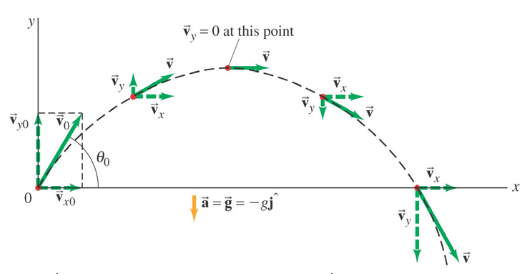
\includegraphics[width=0.7\linewidth]{projectiel}
        \caption{Er zal enkel een in de verticale component een versnelling aanwezig zijn. Hierdoor verandert de snelheid enkel in de verticale component.}
        \label{projectiel}
    \end{figure}
    \begin{table}[h]
        \centering
        \begin{tabular}{|c|c|}
            \hline
            \textbf{Horizontaal}     & \textbf{Verticaal}                        \\
            \hline
            \(a_x = 0\)              & \(a_y = -g\)                              \\
            \hline
            \(v_x(t) = v_{x0}\)      & \(v_y(t) = v_{y0} - gt\)                  \\
            \hline
            \(x(t) = x_0 + v_{x0}t\) & \(y(t) = y_0 + v_{y0}t - \frac{gt^2}{2}\) \\
            \hline
        \end{tabular}
    \end{table}


    \section{Dynamica: Newton's bewegingswetten}
    4.1-4.7

    \subsection{Eerste wet: inertie}
    Een lichaam in rust (of in eenparige rechtlijnige beweging) zal in rust (eenparige rechtlijnige beweging) blijven tenzij er een uitwendige resulterende kracht inwerkt.
    \[\sum_{i}\vec{F_i} = 0 \Rightarrow \vec{a} = 0\]

    \subsection{Tweede wet: versnelling}
    Een grotere kracht op een lichaam met massa m veroorzaakt een grotere versnelling: $a \sim F$

    Bij een dubbele massa 2m zal eenzelfde kracht slechts een versnelling a/2 veroorzaken: $a \sim \frac{1}{m}$

    \[\sum_{i} \vec{F_i} = \vec{F} = m\vec{a}\]

    \subsection{Derde wet: actie-reactie}
    Bij wisselwerking tussen twee lichamen is de kracht \(\vec{F_{21}}\) van lichaam 1 op lichaam 2 even groot en tegengesteld aan de kracht \(\vec{F_{12}}\) van lichaam 2 op lichaam 1.
    \[\vec{F_{12}} = -\vec{F_{21}}\]
    Deze krachten komen steeds in paren voor en werken op verschillende voorwerpen.

    \subsection{Gewicht - Gravitatie - Normaalkracht}
    Alle voorwerpen nabij het aardoppervak vallen met dezelfde versnelling $\vec{g}$.
    \[\text{Gravitatiekracht: } \vec{F_G} = m\vec{g}\]


    \section{De wetten van Newton: wrijving, cirkelbeweging, weerstandskrachten}
    5.1-5.3, 5.5-5.6
    
    \subsection{Wrijvingskrachten}
    Voorwerpen in een ERB duren niet oneindig, de oorzaak hiervan is de wrijvingskracht. Dit is weerstand wanneer een voorwerp
    over het oppervlak van een ander voorwerp beweegt. Deze wrijvingskracht is proportioneel afhankelijk van de normaalkracht
    op een voorwerp $F_{fr} \sim F_{n}$.  De everedigheidsconstante hangt af van de soort wrijvingskracht op een voorwerp.\\
    
    Er zijn twee soorten wrijvingskrachten:
    \begin{enumerate}
            [label=\alph*)]
            \item Kinetische wrijvingskracht
            \item Statische wrijvingskracht
        \end{enumerate}
        
    De nettokracht op een voorwerp is gegeven als volgt:
    
    $$ F_{net} = F_{A} -  F_{fr} $$
    
     \begin{figure}[h]
        \centering
        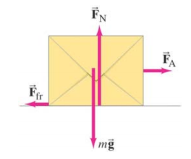
\includegraphics[width=0.3\linewidth]{papierdoos}
        \caption{Verduidelijkende figuur bij wrijvingskrachten}
        \label{papierdoos}
    \end{figure}    
        
    Kinetische wrijvingskracht is de wrijvingskracht die inwerkt op een voorwerp als het voorwerp in beweging is.    
    De grootte van deze wrijvingskracht is afhankelijk van de kinetische wrijvingscoëfficient $\mu_{k}$:
    
   $$ F_{k} = \mu_{k}F_{n} $$
   
   Statische wrijvingskracht is de wrijvingskracht die inwerkt op een voorwerp als het voorwerp nog niet in beweging is.
   De grootte van deze wrijvingskracht is afhankelijk van de statische wrijvingcoëfficient $\mu_{s}$:
   
   $$F_{s} \leq \mu_{s}F_{n}$$
   
   Belangrijk is op te merken dat als het voorwerp in rust staat, de volgende gelijkheid geldt:
   
   $$\vec{F_{s}} = -\vec{F_{A}}$$
   
   In het algemeen is het moeilijker een voorwerp in beweging te krijgen dan het verder te laten bewegen en is dus $\mu_{s} > \mu_{k}$
   
   \subsection{Weerstand en eindsnelheid}
   Als het voorwerp zich doorheen een medium (of fluïda) beweegt, is de wrijvingskracht afhankelijk van de snelheid van het voorwerp.
   Voor relatief kleine voorwerpen met lage snelheid geldt:
   
   $$ \vec{F_{d}} = -b\vec{v} $$
   
   waarbij $b$ een factor is die afhangt van de grootte/vorm van het voorwerp en de viscositeit (of stroperigheid)
   van de vloeistof.
   
   In evenwicht geldt dat de eindsnelheid van een voorwerp gegeven wordt door:
   
   \begin{center}
   	 \[F_{net} = 0\]
	  $\Luda$\[mg - bv_{t} = 0\]
	  $\Luda$\[v_{t} = \frac{mg}{b}\]
    \end{center}	  

    \subsection{Kinematica van de cirkelbeweging}
    Als een voorwerp in een cirkel beweegt, verandert de richting van de snelheid constant. Dit wilt dus zeggen dat:
    
    $$ \vec{a} \neq 0$$
    
    We kunnen de richting als volgt afleiden:
    
    \begin{center}
    	\[\vec{a} = \lim_{\Delta t\to\infty} = \frac{\Delta \vec{v}}{\Delta t} = \frac{d\vec{v}}{dt}\]
    	$\Luda$\\
    	Als $\Delta t$ infinitesimaal klein wordt is $\Delta \vec{v}$ infinitesimaal klein\\
    	$\Luda$\[\Delta\vec{v} \perp \vec{v}\]
    	$\Luda$\[\vec{a} \perp \vec{v}\]
    	$\Luda$\\ 
    	$\vec{a}$ wijst naar het middelpunt van de cirkel.
    \end{center}
    
    De grootte leiden we als volgt af:
    
    \begin{center}
    	\[\vec{a} = \lim_{\Delta t \to 0} = \frac{\Delta \vec{v}}{\Delta t} = \frac{d\vec{v}}{dt}\]
    	$\Luda$\\ Uit de figuur leiden we gelijkvormige driehoeken $1$ en $2$ af
	    	\begin{figure}[h]
	        		\centering
	       		 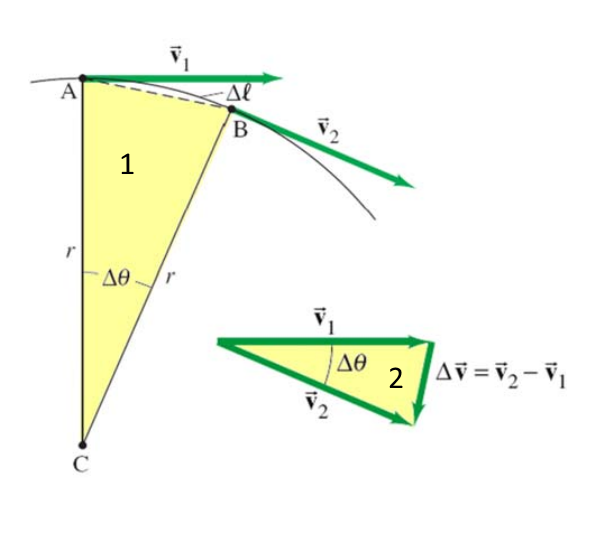
\includegraphics[width=0.6\linewidth]{cirkel}
	       		 \caption{Gelijkvormige driehoeken bij afleiding grootte van de versnelling van een cirkelbeweging}
	        		\label{cirkel}
	    	\end{figure}
	$\Luda$\[\frac{\Delta v}{v} \sim \frac{\Delta l}{r}\]
	$\Luda$\[\Delta v \sim \frac{v\Delta l}{r}\]	    	
	We zien nu dat:
	\[a_{r} = \lim_{\Delta t\to 0} \frac{\Delta v}{\Delta t}\]
	$\Luda$\[a_{r} = \lim_{\Delta t \to 0} \frac{v}{r}\frac{\Delta l}{\Delta t}\]
	$\Luda$\[a_{r} = \frac{v}{r} \lim_{\Delta t \to 0} \frac{\Delta l}{\Delta t}\]
	$\Luda$\[a_{r} = \frac{v^{2}}{r}\]
    \end{center}
    
    We kunnen ook met behulp van volgende begrippen de snelheid van een voorwerp in een cirkelbeweging afleiden:
    \begin{enumerate}
    	\item de periode $T$ = tijd nodig voor 1 omwenteling
    	\item de frequentie $f$ = aantal omwentelingen per seconde (in Hertz)
    \end{enumerate}
    
    We zien dan dat $T = \frac{1}{f}$ en dat:
    
    \begin{center}
    	\[v = 2\pi rf\]	
    \end{center}
    
    \subsection{Dynamica van de cirkelbeweging}
    Er is een kracht nodig om een voorwerp op een cirkelbaan te houden, dit is de centripetale kracht. Deze kracht wijst altijd naar het middelpunt
    van de cirkel en zorgt voor een centripetale versnelling. 
    
    $$ \sum F_{R} = ma_{r} = m\frac{v^{2}}{r} $$ 
    
    Als de centripetale kracht wegvalt, zal door inertie (eerste wet van Newton), het voorwerp gewoon rechtdoor bewegen in plaats van op de cirkelbaan te blijven. 
    De snelheid van een voorwerp kan ook veranderen. Dan heeft de versnelling twee componenten: de radiale component en de tangentiële component. Deze componenten
    kunnen worden gezien als componenten voor de totale versnelling:
    
    \begin{enumerate}
    	\item $a_{r} = \frac{v^{2}}{r}$
    	\item $a_{tan} = \frac{dv}{dt}$
    \end{enumerate}
    
    Dan is de totale versnelling gelijk aan:
    
    $$ a = \sqrt{a_{tan}^{2} + a_{r}^{2}} $$ 
    
    \begin{figure}[h]
    	\centering
	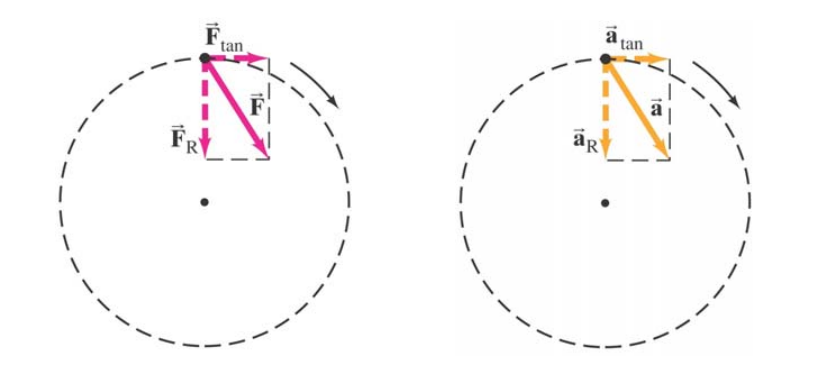
\includegraphics[width=0.6\linewidth]{cirkel_versnelling}
    	\caption{Radiale en tangentiële versnelling bij een cirkelbeweging}
        	\label{cirkel_versnelling}
    \end{figure}

    \section{De zwaartekracht en de synthese van Newton}
    6.1-6.4, 6.6

    \subsection{De wet van de universele zwaartekracht}
    Elk paar van voorwerpen oefent een kracht uit op elkaar. Zo oefent ook de Aarde een kracht uit op andere voorwerpen (vb. de maan). 
    Uit de tweede wet van Newton zien we dat de kracht evenredig is met de massa (1). Uit de derde wet van Netwon
    zien we dan ook dat de kracht evenredig is met de massa van de aarde (2). Uit experimenten halen we ook dat de kracht
    omgekeerd evenredig is met het kwadraat van de afstand tussen de twee voorwerpen (3). 
    
    \begin{enumerate}
    	\item $F \sim m_{voorwerp_{A}}$
    	\item $F \sim m_{voorwerp_{B}}$
    	\item $F \sim \frac{1}{r^{2}}$
    \end{enumerate}
    
    Als we deze 3 eigenschappen combineren vinden we dat de kracht tussen de twee voorwerpen gegeven wordt door:
    
    $$ F \sim \frac{m_{A}m_{b}}{r^{2}} $$

    Elk deeltje in het universum trekt elk ander deeltje aan met een kracht die recht everedig is met het product van hun massa's en omgekeerd
    evenredig is met het kwadraat van hun afstand. Voor de zwaartekracht is de evenredigheidsconstante $G$:
    
    $$ G = 6.673 \times 10^{-11} \frac{Nm^{2}}{kg^{2}} $$ 
    
    Waaruit volgt dat de zwaartekracht $F_{g}$ gedefinieerd is als:
    
    $$ F_{g} = G \frac{m_{A}m_{b}}{r^{2}} $$ 
    
    Belangrijk is te weten dat dit enkel geldt voor puntmassa's! Voor een symmetrische bol of schil, 
    doen we alsof alle massa in één punt zit.
    
    \subsection{Zwaartekracht nabij het oppervlak}
    Als een massa zicht op een hoogte $h$ boven het aardoppervlak bevindt en de straal van de aarde is $R_{a}$, dan is de zwaartekracht op dat voorwerp:
    
    $$ F_{a} = G\frac{mM_{a}}{(R_{a} + h)^{2}} \sim G\frac{mM_{a}}{R_{a}^{2}}$$
    
    We kunnen nu de valversnelling afleiden:
    
    $$ F_{g} = ma $$
    $$\Luda$$
    $$ F_{g} = mg $$
    $$\Luda$$
    $$ mg = G\frac{mM_{a}}{R_{a}^{2}}$$
    $$\Luda$$
    $$ g = G\frac{M_{a}}{R_{a}^{2}} $$
    $$\Luda$$
    $$ g = 9.81 \frac{m}{s^{2}} $$
    
    Aangezien dit berekent is op $h = 0$, kan dit echter afwijken afhankelijk van $h$ als $0 \leq h$. 
    
    \subsection{Satellieten}
    Uit de eerste wet van Newton weten we dat een satelliet zondere kracht rechtdoor zou bewegen. Er werkt echter een kracht in
    op de satelliet, namelijk de gravitatiekracht. We weten dus dat de kracht die inwerkt op de satelliet, de gravitatiekracht, de satelliet
    op zijn baan houdt:
    
    $$ F_{a} = ma $$
    $$\Luda$$
    $$ G\frac{mM_{a}}{r^{2}} = m\frac{v^{2}}{r} $$ 
    $$\Luda$$
    $$ v = \sqrt{\frac{GM_{a}}{r}}$$
    $$\Luda$$
    $$ v = \sqrt{\frac{GM_{a}}{R_{a} + h}} $$
    
    \subsection{Het gravitatieveld}
    Het gravitatieveld is een manier op de impact van de gravitatie in algemene termen weer te geven voor eender welk punt. Het kan gedefinieerd worden met behulp
    van volgende afleiding.
    
    $$ \vec{F_{g}} = -m\vec{a}$$
    $$\Luda$$
    $$ \vec{F_{g}} = -mG\frac{M_{a}}{r^{2}}\vec{u_{r}}$$
    $$\Luda$$
    $$ \vec{F_{g}} = -mg\vec{u_{r}}$$
    $$\Luda$$
    $$ \vec{F_{g}} = m\vec{g}$$
    $$\Luda$$
    $$ \vec{g} = \frac{\vec{F_{g}}}{m}$$
    
    We zien nu dat een massa $m$ die geplaatst wordt op een punt waar het veld gelijk is aan $\vec{g}$ een kracht ondervindt:
    
    $$ \vec{F_{g}} = m\vec{g}$$ 

    \section{Arbeid en Energie}
    7.1, 7.3-7.4 (+14.1)

    \subsection{Arbeid en Energie}
    Het algemene probleem dat optreedt bij de dynamica van een probleem is de tijdsafhankelijkheid.
    We hebben in hoofdstuk 4 gezien dat:
    
    $$ \sum_{i} \vec{F_{i}} = m\frac{d\vec{v}}{dt} = m\vec{a} $$
    
    We zien hier echter dat we een kracht niet kunnen bepalen in functie van de tijd. Daarom voeren
    we de notie in van Arbeid en Energie. De definities zijn als volgt:
    
    \begin{enumerate}
    	\item Een systeem dat in staat is om arbeid te leveren, bezit energie
    	\item Energie is de capaciteit om arbeid te leveren
    	\item Arbeid is de overdracht van energie
    \end{enumerate}
    
    \emph{Opmerking}: Arbeid en Energie zijn gelijkwaardig, ze hebben dezelfde eenheid en dimensie (zie later)
    
    \subsection{Arbeid en Energie door een constante kracht}
    De arbeid geleverd door een kracht is afhankelijk van de efficiëntie van de kracht (grootte en richting) en de afstand waarover de kracht wordt uitgeoefend. 
    Arbeid wordt gedefinieerd als: 
    
    $$ W = F_{\parallel }d = Fd\cos{\theta} = \vec{F} \cdot \vec{d}$$
    
    Een kracht oefent dus géén arbeid uit in de volgende gevallen:
    \begin{enumerate}
    	\item Er is geen verplaatsing
    	\item $\vec{F} \perp \vec{d}$
    \end{enumerate}
    
    De eenheid van arbeid is de Joule ($1J = 1Nm)$.
    
    \subsection{Arbeid langs een pad o.i.v. een variabele kracht}
    Wat als de beweging niet rechtlijnig is en de kracht niet constant zoals in de onderstaande afbeelding?
    
    \begin{figure}[h]
    	\centering
	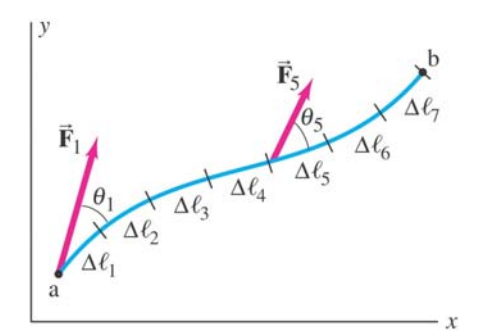
\includegraphics[width=0.6\linewidth]{variabele_kracht}
    	\caption{Variabele kracht langst een pad}
        	\label{variabele_kracht}
    \end{figure}
    
    We delen het pad op in N infinitisimaal kleine deeltjes $\Delta l_i$ met $\vec{F_i}$. De totale arbeid langsheen het pad kan worden gevonden door:
    
    $$\Delta W \sim F_{i}\cos{\theta_{i}}\Delta l_{i}$$
    $$\Luda$$
    $$W \sim \sum_{i = 1}^{N} F_{i}\cos{\theta_{i}}\Delta l_{i}$$
    $$\Luda$$
    $$W = \lim_{\Delta l_{i} \to 0}\sum F_{i}\cos{\theta_{i}}\Delta l_{i}$$
    $$\Luda$$
    $$W = \int_{a}^{b} F\cos{\theta}\Delta l $$ 
    $$\Luda$$
    $$W = \int_{a}^{b} \vec{F} \cdot d\vec{\emph{l}} $$
    
    Dit is algemeen geldig voor elke ruimtedimensie (x, y en z). We kunnen dus in het algemeen schrijven:
    
    \begin{center}
    	$\vec{F} = F_{x}\vec{e_{x}} + F_{y}\vec{e_{y}} + F_{z}\vec{e_{z}}$\\
     	en\\
   	$d\vec{l} = dx\vec{e_{x}} + dy\vec{e_{y}} + dz\vec{e_{z}} $\\
   \end{center}
    $$\Luda$$	
    $$W = \int_{x_{a}}^{x_{b}} F_{x}dx + \int_{y_{a}}^{y_{b}} F_{y}dy + \int_{z_{a}}^{z_{b}} F_{z}dz$$
    
    \subsection{Teruggroepkracht van schroefveren}
    \emph{Opemerking}: Dit is hoofdstuk 14.1 in het handboek!
   
    De teruggroepkracht van een veer (Wet van Hooke): 
    
    $$ F_{x} = -kx $$ 
    
    met $k$ de veerconstante. We kunnen de externe arbeid dan schrijven als:
    
    $$W_{e} = \int_{x_{i}}^{x_{f}} Fds = \int_{-x_{max}}^{0}(-kx)dx = \frac{1}{2}kx^{2}_{max}$$
    
    De arbeid geleverd door de veer is dan:
    
    $$W_{s} = \int_{x_{i}}^{x_{f}} Fds = \int_{0}^{x_{max}}(-kx)dx = -\frac{1}{2}kx^{2}_{max}$$
    
    \subsection{Kinetische Energie}
    We weten uit eerdere hoofdstukken dat:
    
    \begin{enumerate}
    	\item $F_{netto} = ma$
    	\item $a = \frac{v_{2}^{2} - v_{1}^{2}}{2d}$
    \end{enumerate}
    
    We kunnen dan met behulp van de definitie van arbeid afleiden dat:
    
    $$W_{netto} = F_{netto}d$$
    $$\Luda$$
    $$W_{netto} = mad$$
    $$\Luda$$
    $$W_{netto} = m\left( \frac{v_{2}^{2} - v_{1}^{2}}{2} \right)$$
    $$\Luda$$
    $$W_{netto} = \frac{1}{2} mv_{2}^{2} - \frac{1}{2} mv_{1}^{2} $$
    
    We definiëren kinetische energie als: $K = \frac{1}{2}mv^{2}$. We kunnen een analoge afleiding maken voor
    een variabele kracht langst een pad. We zien dan dat:
    
    $$W_{netto} = \int \vec{F_{netto}} \cdot d\vec{l}$$
    $$\Luda$$
    $$W_{netto} = \int F_{netto}\cos{\theta}dl$$
    $$\Luda$$
    $$W_{netto} = \int F_{||}dl$$

    Waarin $F_{||}$ de component van de nettokracht evenwijdig aan de verplaatsing op een willekeurig punt is. Volgens de tweede wet van Netwon is:

    $$F_{||} = ma_{||} = m\frac{dv}{dt}$$

    Waarin $a_{||}$ de component van $a$ evenwijdig aan de kromme op een willekeurig punt, gelijk is aan de snelheid waarmee de snelheid verandert, $\frac{dv}{dt}$. 
    We beschouwen $v$ als een functie van $l$:

    $$\frac{dv}{dt} = \frac{dv}{dl} \frac{dl}{dt} = \frac{dv}{dl}v$$

    Omdat $\frac{dv}{dt}$ de snelheid is geldt:

    $$W_{netto} = \int_{1}^{2} F_{||}dl$$
    $$\Luda$$
    $$W_{netto} = \int_{1}^{2} m\frac{dv}{dt}dl$$
    $$\Luda$$
    $$W_{netto} = \int_{1}^{2} mv\frac{dv}{dl}dl$$
    $$\Luda$$
    $$W_{netto} = \int_{1}^{2} mvdv$$
    $$\Luda$$
    $$W_{netto} = \frac{1}{2} mv_{f}^{2} - \frac{1}{2}mv_{i}^{2} = \Delta K$$
    
    \section{Behoud van energie}
    8.1-8.3, 8.5, 8.8
    
    \subsection{Conservatieve en niet-conservatieve krachten}
    We definiëren een conservatieve kracht als een kracht waarbij de netto arbeid geleverd door deze kracht
    onafhankelijk is van de gevolgde weg. 
    
    We geven hier het voorbeeld van zwaartekracht:
    
    \begin{figure}[h]
    	\centering
	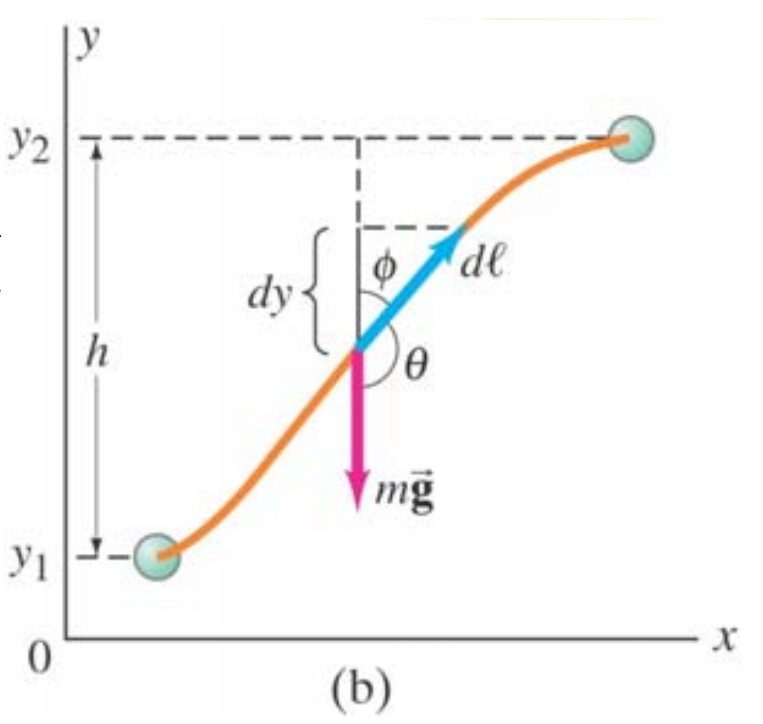
\includegraphics[width=0.6\linewidth]{zwaartekracht_conservatief}
    	\caption{Verduidelijkende figuur bij afleiding}
        	\label{zwaartekracht_conservatief}
    \end{figure}

    We weten dat de gravitatiekracht $\vec{F} = m\vec{g}$. We nemen hier $\vec{F} = -mg\hat{k}$. 
    Dan is de arbeid $W$ gegeven door:
    
    $$W = -\int_{a}^{b}mg\hat{k} \cdot d\vec{r}$$
    $$\Luda$$
    $$W = -mg\int_{a}^{b}\hat{k}\cdot (dx\hat{i} + dy\hat{j} + dz\hat{k})$$
    $$\Luda$$
    $$W = -mg\int_{a}^{b}dz$$
    $$\Luda$$
    $$W = -mg(z_b - z_a)$$

    Hier zien we dat de arbeid geleverd inderdaad alleen afhankelijk is van begin en eindpunt. Een andere manier waarop
    we een conservatieve kracht kunnen definiëren is de volgende: Een kracht is conservatief wanneer de netto arbeid geleverd
    door deze kracht gelijk is aan nul bij een gesloten baan. 
    
    \subsection{Potentiële Energie}
    Potentiële energie kan men samenvatten als een fenomeen waarbij energie wordt opgeslagen. Zo kunnen we bijvoorbeeld
    de gravitationele potentiële energie beschrijven als:
    
    $$\Delta U_g = W_{ext} = -W_{gravitatie} = mg(h_2 - h_1)$$
    
    Belangrijk is echter het verschil in potentiële energie. Potentiële energie op zich heeft geen betekenis (het is relatief t.o.v.
    begin en eindpunt). Over het algemeen geldt voor conservatieve krachten:
    
    $$W = \int_{1}^{2}\vec{F}\cdot d\vec{r} = U_1 - U_2 = -\int_{1}^{2} U$$
    
    We zien dus dat de arbeid geleverd door een conservatieve kracht gelijk is aan het tegengestelde van de verandering in potentiële energie. We kunnen
    dit uitbreiden naar 3 dimensies:
    
    \begin{enumerate}
    	\item $F_x = -\frac{\delta U}{\delta x}$
    	\item $F_y = -\frac{\delta U}{\delta y}$
    	\item $F_z = -\frac{\delta U}{\delta z}$
    \end{enumerate}
    
    En dus is $\vec{F} = -grad(U) = -\mathbb{\nabla}{U}$.

    \subsection{Behoud van mechanische energie}
    De totale mechanische energie van een deeltje: $E = K + U$,
    blijft constant als de inwerkende krachten conservatief zijn.
    
    Als er niet-conservatieve krachten mee inwerken op het deeltje, 
    is de arbeid van alle niet-conservatieve krachten gelijk aan de verandering
    in mechanische energie: $W = \Delta E$. Deze twee beweringen vormen
    samen de wet van behoud van energie.
    
    \subsection{Vermogen}
    Vermogen geeft weer in welk tempo er arbeid wordt verricht. Het gemiddelde vermogen is
    $P_{gem} = \frac{W}{\Delta t}$. Net zoals snelheid, versnelling, etc, kunnen we het ogenblikkelijke vermogen
    schrijven als:
    
    $$P = \frac{dW}{dt} = \frac{dE}{dt}$$
    
    Of via de definitie van arbeid:
    
    $$P = \vec{F} \cdot \frac{d\vec{r}}{dt} = \vec{F} \cdot \vec{v}$$ 
    
     Vermogen wordt uitgedrukt in Watt: $1 \frac{J}{s} = 1 W$.

    \section{Impuls}
    9.1-9.2 (+36.11, 42.4)

    \subsection{Impuls}
    De impuls is een manier om de hoeveelheid beweging van een een voorwerp te
    bepalen. Het wordt ook lineair momentum genoemd. Hoe meer impuls een voorwerp
    heeft, hoe meer impact het voorwerp zal hebben op andere voorwerpen. We zullen
    ook zien dat er een kracht nodig is om de impuls van een voorwerp te veranderen. We
    definiëren de impuls als:
    
    $$\vec{p} = m\vec{v}$$
    
    We kunnen nu ook de tweede wet van Newton herschrijven:
    
    $$\sum \vec{F} = \frac{d(m\vec{v})}{dt} = \frac{d\vec{p}}{dt}$$

    \subsection{Behoud van impuls}
    Stel twee deeltjes in een geïsoleerd systeem voor waarbij:
    
    $$\vec{F_{21}} + \vec{F_{12}} = 0$$
    
    En waarbij volgens de tweede wet van Newton geldt dat $\vec{F_{21}} = \frac{d\vec{p_1}}{dt}$ en 
    $\vec{F_{12}} = \frac{d\vec{p_2}}{dt}$. Dan vinden we dat:
    
     $$\vec{F_{21}} + \vec{F_{12}} = 0$$
     $$\Luda$$
     $$\frac{d\vec{p_1}}{dt} + \frac{d\vec{p_2}}{dt} = 0$$
     $$\Luda$$
     $$\frac{d}{dt}(\vec{p_1} + \vec{p_2}) = 0$$
     $$\Luda$$
     $$p = (\vec{p_1} + \vec{p_2}) = cte$$

    We zien dus dat de totale impuls van een geïsoleerd systeem constant is. 

    \section{Rotatie}
    10.1, 10.4, 10.8
    
    \subsection{Grootheden bij rotatie}
    Een hoekverplaatsing $\Delta \theta$ wordt gegeven door:
    
    $$\Delta \theta = \theta_{2} - \theta_{2}$$
    
    Een hoek wordt gedefinieerd als:
    
    $$\theta = \frac{l}{R}$$ 
    
    waarbij $R$ de radius is van een cirkel en $l$ een booglengte op die cirkel. Net zoals bij kinematica kunnen we de begrippen
    snelheid invoeren, dit maal als gemiddelde en ogenblikkelijke hoeksnelheid (resp.):
    
    $$\omega_{gem} = \frac{\Delta \theta}{\Delta t}$$
    $$\omega = \lim_{\Delta t \to 0} \frac{\Delta \theta}{\Delta t} = \frac{d\theta}{dt}$$
    
    De eenheid van hoeksnelheid is radialen / seconde (of kortweg rad/s). We kunnen met behulp van de hoeksnelheid
    (die hetzelfde is voor elk punt in het object) ook de lineaire snelheid bepalen. De lineaire snelheid is voor punten dichter
    bij de rotatie-as kleiner als voor punten verder weg van de rotatie-as, aangezien deze een kleinere booglengte $l$
    moeten afleggen om dezelfde hoekverplaatsing $\Delta \theta$ af te leggen:
    
    $$\omega = \frac{d\theta}{dt} = \frac{1}{R} \frac{dl}{dt} = \frac{v}{R}$$
    $$\Luda$$
    $$v = \omega R$$

    \subsection{Krachtmoment}
    Wat als er een kracht inwerkt op een punt $P$ met massa $m$. Het moment van de kracht $F$ 
    t.o.v. de oorsprong van het referentiestelsel is gegeven door:
    
    $$\vec{\tau} = \vec{r} \times \vec{F}$$
    
    Dit moment van de kracht is de tendens van een kracht om de draaibeweging van een voorwerp
    te veranderen.  De eenheid van dit moment is $Nm = J$. 
    
    \subsection{Arbeid en energie bij rotatie}
    In hoofdstuk $7$ (deel $10$) is de kinetische energie van een object gedefinieerd als: $K = \frac{1}{2}mv^{2}$. We
    hebben echter gezien dat $v$ bij rotatie verschillend is voor ieder punt, afhankelijk van hoever ze zich bevonden van
    de rotatie-as. Stel dat we het object onderverdelen in kleine massa's $m_i$ elk met een (lineaire) snelheid $v_i$, dan kunnen
    we de kinetische energie voor een object met rotatie afleiden als:
    
    $$K = \sum \left( \frac{1}{2} m_{i} v_{i}^{2}\right)$$
    $$\Luda$$
    $$\omega \textrm{ is gelijk voor elke massa } m_{i}$$
    $$\Luda$$
    $$K = \sum \left( \frac{1}{2} m_{i} R_{i}^{2}\omega^{2}\right)$$
    $$\Luda$$
    $$K = \frac{1}{2} I\omega^{2} \textrm{ met het traagheidsmoment } I = \sum \left(m_{i} R_{i}^{2}\right)$$
    
    De arbeid die geleverd wordt kunnen we ook gemakkelijk afleiden:
    
    $$W = \int \vec{F} \cdot d\vec{l}$$
    $$\Luda$$
    $$W = \int F_{\perp}Rd\theta$$
    $$\Luda$$
    $$W = \int_{\theta_{1}}^{\theta_{2}} \tau d\theta$$

    \section{Impulsmoment}
    11.3-11.4, 11.6
    \subsection{Impulsmoment}
    Het impulsmoment van een deeltje met massa $m$ op plaats $P$ wordt gegeven als:
    
    $$\vec{L} = \vec{r} \times \vec{p}$$
    
    waarbij $\vec{r}$ de positievector is van het deeltje en $\vec{p}$ de impuls gezien in hoofdstuk $9$ (deel $11$).
    Het impulsmoment geeft de tendens van het deeltje weer om rond de oorsprong $O$ te draaien. We zien ook dat dankzij
    het kruisproduct:
    
    \begin{enumerate}
    	\item als $r \perp p \to L = mvr$ (L is maximaal)
    	\item als $r \parallel p \to L = 0$
   \end{enumerate}
   
   Een andere belangrijke bevinding is dat:
   
   $$L = mvr$$
   $$\Luda$$
   $$L = m(\omega r)r$$
   $$\Luda$$
   $$L = m\omega r^{2}$$
   $$\Luda$$
   $$L = I\omega$$
   
   \subsection{Verband tussen impulsmoment en krachtmoment}
   We zullen net zoals bij impuls bewijzen dat het impulsmoment van een voorwerp geconserveerd is:
   
   $$\vec{L} = \vec{r} \times \vec{p}$$
   $$\Luda$$
   $$\frac{d\vec{L}}{dt} = \frac{d\vec{r}}{dt} \times \vec{p} + \vec{r} \times \frac{d\vec{p}}{dt}$$
   $$\Luda$$
   $$\vec{L} = \vec{v} \times \vec{p} + \vec{r} \times \vec{F} \textrm{ (Zie impuls)}$$
   $$\Luda$$
   $$\vec{L} = \vec{r} \times \vec{F} = \vec{\tau} $$
   
   We zien dus enkele verbanden, namelijk dat:
   
   \begin{enumerate}
   	\item $\vec{F} = \frac{d\vec{p}}{dt}$
   	\item $\vec{\tau} = \frac{d\vec{L}}{dt}$
   \end{enumerate}

    Wie zien dus dat een kracht de impuls van een voorwerp verandert (de hoeveelheid beweging van een systeem verandert) en dat
    een krachtmoment (a.k.a. torsie) het impulsmoment van een voorwerp verandert (de hoeveelheid draaibeweging van een systeem verandert).
    
    \subsection{Behoud van impulsmoment}
    Neem twee deeltjes in een geïsoleerd systeem, d.w.z. er zijn geen externe krachten die inwerken op de deeltjes:
    We weten dankzij de tweede wet van Newton dat:
    
    $$\vec{F_{12}} + \vec{F_{21}} = 0$$
    
    en we weten ook dat:
    
    $$\frac{d\vec{L_{1}}}{dt} = \vec{\tau_{1}} \textrm{ en } \frac{d\vec{L_{2}}}{dt} = \vec{\tau_{2}}$$

    We leiden af:
    
    $$\tau_1 + \tau_2 = \vec{r_{1}} \times \vec{F_{12}} + \vec{r_{2}} \times \vec{F_{21}}$$
    $$\Luda$$
    $$\tau_1 + \tau_2 = (\vec{r_{2}} - vec{r_{1}}) \times \vec{F_{21}} = 0$$
    $$\Luda$$
    $$\frac{d\vec{L_{1}}}{dt} + \frac{d\vec{L_{2}}}{dt} = \frac{d}{dt}(\vec{L_1} + \vec{L_2}) = 0$$
    
    Het totale impulsmoment tussen twee deeltjes blijft dus constant in grootte en in richting.
    
    
    \section{Pollevs}
    \begin{itemize}
    \renewcommand\labelitemi{--}
    \item Een kanonbal volgt pad B op aarde. Welk pad zou de kanonbal op de maan volgen (\(g_{maan} = 1.6m/s^2\)) indien hij op dezelfde manier uit het kanon werd afgevuurd? (zie afbeelding cursus)
    \begin{enumerate}
    	[label=\alph*)]
    	\item A
    	\item B
    	\item C
    	\item D
    \end{enumerate}
    \textit{Oplossing:} D, g is kleiner dus de versnelling naar beneden is kleiner.
    \newline
    \item Welk van de volgende stellingen is het meest correct?
    \begin{enumerate}[label=\alph*]
    	\item Het is mogelijk dat een voorwerp in beweging is zonder dat er krachten op het voorwerp werken.
    	\item Het is mogelijk dat er krachten op een voorwerp inwerken zonder dat er beweging is.
    	\item A en B zijn fout.
    	\item A en B zijn correct.
    \end{enumerate}
    \textit{Oplossing:} A en B zijn beide correct. Een voorwerp A) Een voorwerp op een trein, het beweegt tegenover de aarde. B) Een voorwerp dat op een bank ligt, maar zwaartkracht werkt hier wel op in.
    \newline
    \item Een voorwerp ondervindt een nettokracht wordt hiervoor versneld. Welke stelling is \textit{altijd} vorrect?
    \begin{enumerate}[label=\alph*]
    	\item Het voorwerp beweegt in de richting van de nettokracht.
    	\item De versnelling is in dezelfde richting als de snelheid.
    	\item De versnelling is in dezelfde richting als de kracht.
    	\item De snelheid van het voorwerp neemt toe.
    \end{enumerate}
    \textit{Oplossing:} d is de juiste oplossing. $\vec{F}$ en $\vec{a}$ hebben gelijke richting en zin op een constante na: \(\vec{F} = m\vec{a}\). Tegenvoorbeeld voor A en B: Het voorwerp is al in beweging en er werkt een kracht loodrecht op dat voorwerp. Tegenvoorbeeld voor C: Als versnelling in tegengestelde richting staat (vertragen).
    \newline
    \item Wanneer een vlieg botst met de voorruit van een snelrijdende bus, welk voorwerp ondervindt dan de grootste impactkracht?
    \begin{enumerate}[label=\alph*]
    	\item De vlieg
    	\item De bus
    	\item Beide ondervinden dezelfde kracht.
    \end{enumerate}
    \textit{Oplossing:} Ze ondervinden beide dezelfde kracht. Dit volgt onmiddelijk uit de 3e wet van Newton: Actie-Reactie. 
    \newline
    \item Wanneer een vlieg botst met de voorruit van een snelrijdende bus, welk voorwerp ondervindt dan de grootste vernselling?
    \begin{enumerate}[label=\alph*]
    	\item De vlieg
    	\item De bus
    	\item Beide ondervinden dezelfde versnelling
    \end{enumerate}
    \textit{Oplossing:} De vlieg zal de grootste versnelling ondervinden. 
    \newline
    \item Je plaatst jouw fysicaboek op een houten plank. Daarna til je één uiteinde van de plank op, zodat de hoek met de tagel toeneemt. Uiteindelijk gaat het boek glijden op de plank. Wanneer je de hoek tussen de plank en de tafel constant houdt op deze waarde, zal het boek
    \begin{enumerate}[label=\alph*]
    	\item met constante snelheid bewegen.
    	\item vertragen.
    	\item vernsellen.
    	\item Geen deze antwoorden is correct. 
    \end{enumerate}
	\textit{Oplossing:} Het boek zal versnellen. Het boek beweegt pas wanneer \(F_z > F_k\). Er blijft een resulterende kracht en versnelling zijn. 
	\newline
	\item Een auto (met kale banden!) rijdt doorheen een cirkelvormige bocht, met de grootste snelheid waarbij de centripetale kracht die nodig is om de auto in een cirkel te laten bewegen, net gelijk is aan de maximale statische wrijvingskracht tussen de banden en de weg. Bij punt P rijdt de auto door een plas, waardoor de staticshe wrijvingscoëfficiënt afneemt. De auto glijdt, waardoor nu kinetische wrijving op de auto werkt. De \textit{richting van deze kinetische wrijvingskracht} is
	\begin{enumerate}[label=\alph*]
		\item in dezelfde richting van de oorspronkelijke statische wrijvingskracht.
		\item in de tegenovergestelde richting van de oorspronkelijke statische wrijvingskracht.
		\item loodrecht op de oorspronkelijke statische wrijvingskracht.
		\item onder 45\degree georienteerd ten opzichte van de oorspronkelijke statische wrijvingskracht.
	\end{enumerate}
	\textit{Oplossing:} Het juiste antwoord is c. De kinetische wrijving zal wijzen naar achter tegenover de auto terwijl de statische wrijvingskracht wees naar het middelpunt van de bocht. 
	\newline
	\item Captain America staat op de top van een zeer hoge berg en gooit een baseball in de horizontale richting, met een zodanige snelheid dat de baseball in een baan rond de aarde gaat bewegen. Wanneer de baseball in deze baan beweegt, is zijn versnelling
	\begin{enumerate}[label=\alph*]
		\item afhankelijk van hoe snel de baseball geworpen werd.
		\item een beetje kleiner dan \(9.81 m/s^2\).
	 	\item gelijk aan \(9.81 m/s^2\).
	 	\item gelijk aan nul omdat de bal niet op de grond valt. 
	\end{enumerate}
	\textit{Oplossing:} Het juiste antwoord is b. De gravitatieversnellling is: \(g = \frac{M_a}{R_a^2}\). De straal zal in dit geval de straal zijn van de aarde + de hoogte van de berg waardoor de valversnelling lager zal liggen dan gewoonlijk. 
	\newline
	\item De gravitatiekracht uitgeoefend door de zon op de aarde, houdt de aardein haar baan rond de zon (neem aan dat de baan een perfecte cirkel is). De arbeid geleverd door de de gravitatiekracht in een zeer kort tijdsinterval, waarbij de aarde een infinitesimale verplaatsing maakt, is
	\begin{enumerate}[label=\alph*]
		\item positief
		\item negatief
		\item nul
		\item onmogelijk te bepalen
	\end{enumerate}
	\textit{Oplossing:} Het antwoord zal nul zijn. De kracht en verplaatsing staan loodrecht op elkaar. 
	\newline
	\item Met een speelgoedpistool kan je pijltjes wegschieten door eerst met het pijltje de veer van het pistool in te drukken over een afstand d. Voor een tweede schot druk je de veer over een afstand 2d in. Hoeveel sneller vliegt het tweede pijltje ten opzichte van het eerste pijltje?
	\begin{enumerate}[label=\alph*]
		\item Vier maal zo snel.
		\item Twee maal zo snel.
		\item Even snel.
		\item Half zo snel.
		\item Een vierde zo snel.
	\end{enumerate}
	\textit{Oplossing:} b is de juiste oplossing hier. De veer wordt verder ingedrukt en dus zal het kogetlje sneller gaan dan de vorige keer. We passen behoud van energie toe: \(W = \frac{kx^2}{2} = \frac{k(2x^2)}{2} = 2kx^2\). Hieruit volgt: \(K = \frac{mv^2}{2} = \frac{4mv^2}{2} = 2mv^2\) en dus is de snelheid verdubbeld.
	\newline
	\item Wat is de betekenis van de helling van een U(x) grafiek?
	\begin{enumerate}[label=\alph*]
		\item De grootte van de kracht op het voorwerp.
		\item Het negatieve van de grootte van de kracht. 
		\item De x-component van de kracht op het voorwerp. 
		\item Het negatieve van de x-component van de kracht op het voorwerp. 
	\end{enumerate}
	\textit{Oplossing:} De hellling is de afgeleide van de potentiële energie tegenover x, dus: \(F_x = -\frac{dU}{dx}\)
	\newline
	\item Een blok met massa m wordt op een horizontaal oppervlak geschoven met beginsnelheid v. Het blok glijdt tot het tot stilstand komt door de wrijving met het oppervlak. Hetzelfde blok wordt nu geschoven op het horizontaal oppervlak, met beginssnelheid 2v. Het blok komt tot rust op een afstand (ten opzichte van de afstand in het eerste geval):
	\begin{enumerate}[label=\alph*]
		\item die gelijk is.
		\item die tweemaal zo groot is.
		\item die viermaal zo groot is.
		\item het is niet mogelijk om het verband te bepalen. 
	\end{enumerate}
	\textit{Oplossing:} c is het juiste antwoord. De wrijving blijft gelijk en er is geen potentiële energie in het systeem. \(E_k^i = \frac{mv^2}{2}\) is wat geldt voor de initiële toestand terwijl in de tweede toestand geldt: \(E_k^f = \frac{m(2v)^2}{2} = 4\frac{mv^2}{2}\)
	\newline
	\item Een auto van een oud model trekt op van rust tot een snelheid v in 10 seconden. Een nieuwer, kachtiger model versnelt van rust tot 2v in dezelfde tijd. Wat is de verhouding van het vermogen van de nieuwe auto ten opzichte van de oudere auto? 
	\begin{enumerate}[label=\alph*]
		\item 0.25
		\item 0.5
		\item 1
		\item 2
		\item 4
	\end{enumerate}
	\textit{Oplossing:} de oplossing is in dit geval 4. \(P = \frac{dW}{dt}\) waarbij de tijd in beide gevallen hetzelfde is, enkel de verhouden van arbeid moet dus berekend worden. \(\frac{W_1}{W_2} = \frac{m(2v)^2}{2} / \frac{mv^2}{2} = 4\).
	\newline 
	\item Een auto en een grote vrachtwagen met dezelfde snelheid botsen frontaal en haken in elkaar vast. Welk voertuig ondervindt de grootste verandering van de impulsgrootte?
	\begin{enumerate}[label=\alph*]
		\item De auto.
		\item De vrachtwagen
		\item Beide ondervinden dezelfde verandering van impulsgrootte.
		\item Het is onmogelijk dit te bepalen. 
	\end{enumerate}
	\textit{Oplossing:} Het antwoord is c. De totale impuls blijft gelijk, wat erbij komt bij de ene zal er bij de andere af gaan. Ze worden 1 systeem na de botsing, de massa neemt toe maar de snelheid blijft gelijk. Impuls van de auto zal evenveel toenemen als deze bij de vrachtwagen afneemt. 
	\newline
	\item Wanneer het niet lukt om een schroef, die zeer vast zit in een plank, los te maken, neem je best een schroevendraaier die
	\begin{enumerate}[label=\alph*]
		\item langer is.
		\item dikker is.
		\item noch A, noch B maakt iets uit.
	\end{enumerate}
	\textit{Oplossing:} Het is voordeliger als de schroevendraaier dikker is, aangezien dan je momentarm groter is. 
	\newline
	\item Een schaatster nadert een paal en grijpt die vast. Hierdoor draait ze in een cirkel rond de paal. Hoe groot is haar impulsmoment ten opzichte van de paal op het ogenblik dat ze zich op een afstand d van de paal bevindt, en schaatst met een snelheid v langsheen een rechte lijn die paal op een afstand a passeert?
	\begin{enumerate}[label=\alph*]
		\item Nul
		\item mvd
		\item mva
		\item Onmogelijk te bepalen. 
	\end{enumerate}
	\textit{Oplossing:} Het antwoord is c. \(\vec{L} = \vec{r} \times \vec{p} = d sin\theta m v = amv\)
	\newline
	\item Je vult een emmer tot de helft met water, en vriest het in. Dan roteer je de emmer op een wrijvingsloos platform. Wanneer het ijs smelt, zal de hoeksnelheid van de emmer
	\begin{enumerate}[label=\alph*]
		\item toenemen.
		\item afnemen.
		\item constant blijven.
		\item toe - of afnemen afhankelijk van de hoeveelheid ijs die gesmolten is. 
	\end{enumerate}
	\textit{Oplossing:} b is het antwoord. Het ijs smelt dus wordt de momentarm groter. Een andere uitleg is dat het traagheidsmoment zal vergroten en dus de hoeksnelheid zal afnemen. 
	\end{itemize}
    \newpage


    \section{Deel 2 - Elektriciteit}


    \section{Elektrische velden}
    21.1-21.2, 21.4-21.11, 21.13
	\subsection{Eigenschappen van elektrische lading}
	Er bestaan 2 soorten ladingen: positief en negatief. Tegengestelde ladingen trekken elkaar aan en gelijke ladingen stoten elkaar af. De totale lading van een geisoleerd systeem blijft altijd gelijk. Beweegelijkheid van elektronen hangt af van het materiaal:
	\begin{itemize}
		\item \textit{geleider}: sommige elektronen zijn "vrij" (ongebonden) te bewegen
		\item \textit{isolator}: alle elektronen zijn gebonden, bijgevolg onbeweeglijk
		\item  \textit{halfgeleider}: ergens tussenin
	\end{itemize}
	
	\subsection{Elektrische ladingen door inductie}
	Het opladen van een object via inductie gaat als volgt:
	\begin{figure}[h]
		\centering
		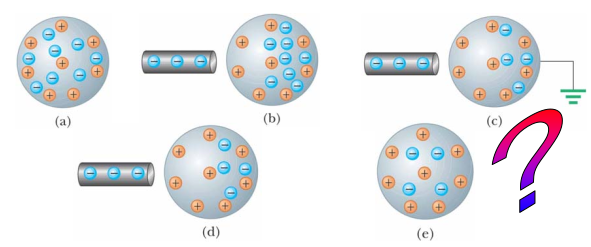
\includegraphics[width=0.7\linewidth]{inductie}
		\label{inductie}
	\end{figure}
	Als er een negatief geladen staaf in de buurt wordt gebracht van een neutraal geladen voorwerp, zullen de elektronen binnen dat voorwerp weggaan naar de aarde en zal het voorwerp uiteindelijk positief geladen zijn. 
	
	\subsection{De wet van Coulomb}
	\[\vec{F}_12 = k_e\frac{q_1 q_2}{r^2}\hat{r} = \frac{q_1q_2}{4\pi \epsilon_0 r^2}\hat{r}\]
	met r de afstand tussen de ladingen. \(\hat{r}\) is de eenheidsvector van $q_1$ naar $q_2$.
	$k_e$ is de \textbf{Coulomb constante} en is gelijk aan \(\frac{1}{4\pi\epsilon_0}\). $\epsilon_0$ is hier de permitiviteit van het vacuum.
	
	Deze kracht is een conservatieve kracht, de weg van het begin tot het einde maakt niet uit. 
	\newline
	
	\subsection{Superpositie van krachten}
	\begin{itemize}
		\item \textit{Discrete ladingsverdeling} 
		\[\vec{F}_{q^*} = \vec{F}_{21} + \vec{F}_{31} + \vec{F}_{41} + ... = k_eq^*\sum_i \frac{q_i}{r_i^2}\hat{r}_i\]
		\item \textit{Continue ladingsverdeling}
		\[\vec{F}_{q^*} = k_eq^* \int\frac{1}{r^2}\hat{r}dq\]
	\end{itemize}
    Deze formule lijkt enorm op de gravitatiekracht. Het grootste verschil is dat de gravitatie altijd aantrekken is terwijl de Coulombkrach afstotend kan zijn.
    
    \subsection{Het elektrisch veld}
    Een elektrisch veld is een veldkracht (dat werkt zonder contact door een lege ruimte) die veroorzaakt wordt door een bronlading Q.
    
    De elektrische veld vector E in een punt in de ruimte is gelijk aan de elektrische kracht $F_e$ die op een \textit{positieve} testlading, gedeeld door de testlading.
    
    \[\vec{E} = \frac{\vec{F}_e}{q_0^*}\]
    
    In de omgezette formule: \(\vec{F}_e = q\vec{E}\) mag de testlading wel negatief zijn. 
    
    \textit{Elektrisch veld tegenover puntlading}:
    \[E = \frac{F}{q} = \frac{kqQ/r^2}{q} = k\frac{Q}{r^2}\]
    Voor meerdere puntladingen geldt dan: \(\vec{E} = k_e \sum_i \frac{q_i}{r_i^2}\hat{r}_i\)
    
    \subsection{De elektrische dipool}
    Een dipool is een positieve lading q en een negatieve lading -q op een afstand $2a$ van elkaar. Stel dat we het elektrische
    veld in een p:

    \begin{figure}
	\centering
	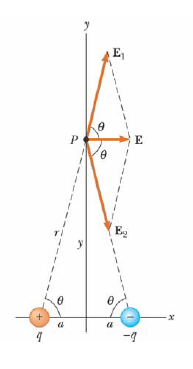
\includegraphics[width=0.3\linewidth]{dipool_elektrische_veld}
	\label{dev}
    \end{figure}

    We kunnen het elektrisch veld als volgt bepalen:

    $$\vec{E} = \vec{E_{1}} + \vec{E_{2}}$$

    en we weten dat:

    $$E_{1} = E_{2} = k_{e} \frac{q}{r^{2}} = k_{e}\frac{q}{y^{2} + a^{2}}$$


    De y-componenten zullen elkaar altijd opheffen, voor de x-componenten geldt:

    $$E = 2E_{1}\cos(\theta) = 2k_{e}\frac{q}{y^{2} + a^{2}}\frac{a}{(y^{2} + a^{2})^{\frac{1}{2}}}$$
    $$\Luda$$
    $$E = k_{e}\frac{2qa}{(y^{2} + a^{2})^{\frac{3}{2}}}$$
    $$\Luda$$
    $$y >> a \to E \sim k_{e}\frac{2qa}{y^{3}}$$

    \subsection{Elektrisch veld van een continue ladingsverdeling}
	Dit is gelijkaardig een heel veel puntladingen. 
	\[\vec{E} = k_e\int\frac{dq}{r^2}\hat{r}\]
	definieer (uniforme) \textit{ladingsverdeling}:
	\begin{itemize}
		\item \textbf{Volume-ladingsverdeling}
		 \[\rho = Q/V \text{ of } dq/dV [C/m^3]\]
		\item \textbf{Oppervlakte-ladingsverdeling}:
		 \[\sigma = Q/A \text{ of } dq/dA [C/m^2]\]
		\item \textbf{Lineaire-ladingsverdeling}:
		 \[\lambda = Q/l \text{ of } dq/dl [C/m]\]
	\end{itemize}
	\subsection{Elektrische veldlijnen}
	Eigenschappen van elektrische veldlijnen:
	\begin{itemize}
		\renewcommand\labelitemi{--}
		\item Het elektrisch veld is een vectorveld
		\item De elektrische veldvector raakt aan de elektrische veldlijn.
		\item Het aantal veldlijnen per oppervlakte-eenheid is evenredig met de elektrische veldsterkte in het beschouwde gebied.
		\item Veldlijnen beginnen bij positieve ladin en eindigen bij negatieve lading.
		\item het aantal lijnen nabij lading is evenredig met de lading.
		\item veldlijnen kunnen nooit kruisen. Als ze dit wel doen, zouden er twee verschillende elektrische velden in 1 punt. 
	\end{itemize}
	\subsection{Beweging van een lading in een uniform veld}
	\[\vec{F}_e = q\vec{E} = m\vec{a} \text{  of  } \vec{a}=\frac{q\vec{E}}{m}\]
	Bij een uniform elektrisch veld is de \textit{versnelling constant}!
	\begin{figure}[h]
		\centering
		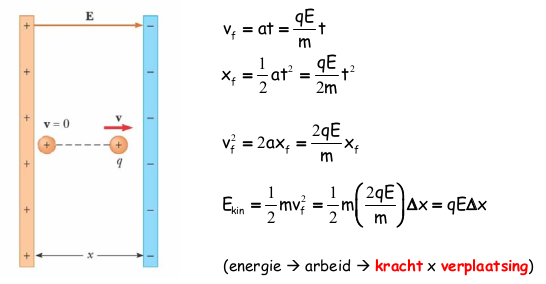
\includegraphics[width=0.7\linewidth]{uniform-elektrisch-veld}
		\label{fig:uniform-elektrisch-veld}
	\end{figure}
	Als het uniform elektrisch veld op zijn zij gaat liggen, zal de elektron een projectielbeweging nabootsen. De versnelling is dan al volgt: 
	\[\vec{a}=-\frac{eE}{m_e}\vec{j}\]
	
	De kracht zal dan de kracht zijn dat het elektrisch veld uitoefent op de elektron. Bij een proton zijn de min in de formule wegvallen. 
	
	\subsection{Beweging van dipool in uniform elektrisch veld}
	\textit{elektrisch dipool}: systeem van 2 even grote ladingen met tegengesteld teken op afstand l.
	Het dipoolmoment is als volgt gedefinieerd: \(\abs{\vec{p}} = Ql\)
	\begin{figure}[h]
		\centering
		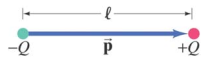
\includegraphics[width=0.3\linewidth]{dipool}
		\label{fig:dipool}
	\end{figure}

	De \textit{totale kracht} op een elektrische dipool in een homogeen veld: 

	\(\vec{F} = \vec{F}_+ + \vec{F}_- = Q\vec{E} - Q\vec{E} = 0\).
	
	\textit{krachtmoment} op een elektrische dipool (rond middelpunt) wordt als volgt gedefinieerd:
	\begin{figure}[h]
		\centering
		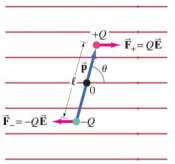
\includegraphics[width=0.4\linewidth]{dippoolmoment}
		\label{fig:dippoolmoment}
	\end{figure}
	\newpage
	\[\tau = QE\frac{l}{2}\sin\theta + QE\frac{l}{2}\sin\theta = pE\sin\theta\]	
	DUS : \(\vec{\tau} = \vec{p} \times \vec{E}\)
	
	\textit{arbeid} geleverd door een elektrisch veld op een elektrische dipool:
	\[W = \int_{\theta_1}^{\theta_2}\tau d\theta = -pE\int_{\theta_1}^{\theta_2}\sin\theta d\theta = pE(\cos\theta_2 - \cos\theta_1) = -\Delta U\]
	DUS: \(U = -\vec{p} \cdot \vec{E}\)
	
	Er is nog een toepassing op het einde van het hoofdstuk, p582 in de Giancoli
	
    \section{De wet van Gauss}
    22.1-22.3

    \subsection{Elektrische flux}
    De elektrische flux is gedefinieerd als het product van de grootte van het elektrisch veld met het oppervlak. Anderzijds is het ook het aantal veldlijnen door het oppervlak. 
    \[\Phi_E = EA' = EA\cos\theta\]
    Waarbij A' staat voor wanneer het elektrisch veld en het oppervlak loodrecht staan op elkaar. Dit is ook allemaal gedefinieerd als het elektrisch veld uniform is, maar kan ook gedefinieerd worden voor een niet-uniform elektrisch veld.
    
    \[\Phi_E = \lim_{\Delta A_i \rightarrow 0} \sum \vec{E}_i \cdot \Delta\vec{A}_i = \int_{\text{surface}} \vec{E}\cdot d\vec{A}\]
    
    De flux zal men hier definiëren over een klein stukje $\Delta A$ van het totale oppervlak A. De vector $d\vec{A}_i$ wordt gedefinieerd als de vector loodrecht op het oppervlak, met de richting van binnen naar buiten.
    
    Om de elektrische flux van een gesloten oppervlak te bepalen kijken we opnieuw naar de definitie: \textbf{netto flux} is het netto aantal veldlijnen dat het oppervlak verlaat. Bij een gesloten oppervlak zullen evenveel lijnen het oppervlak binnentreden als het verlaten, dus is de nettoflux van een gesloten oppervlak altijd nul. De veldlijnen die binnenkomen zorgen voor negatieve flux en de veldlijnen die het oppervlak verlaten zorgen voor positieve flux.
    
    \subsection{De wet van Gauss}
    \textit{Verband tussen flux en ingesloten lading bij gesloten oppervlak}
    
    De grootte van het elektrisch veld voor een puntlading is \(E = k_e q/r^2\) en de veldlijnen wijzen van binnen naar buiten. Er zal dus positieve flux ontstaan. 
   	\[\vec{E}\cdot\Delta A_i = E\Delta A_i \text{  of  } \Phi_E = \int\vec{E}\cdot\vec{A} = \int EdA = E\int A\]
   	\[\Phi_E = k_e\frac{q}{r^2}\cdot 4\pi r^2 = 4\pi k_eq \text{  en  } k_e = \frac{1}{4\pi\epsilon_0} \text{  ,dus  } \Phi_E = \frac{q}{\epsilon_0}\]
   	
   	Dus de nettoflux door een willekeurig gesloten oppervlak dat een lading q omsluit, is steeds gelijk aan $q/\epsilon_0$
   	
   	\textit{Verband tussen flux en lading buiten een gesloten oppervlakte}
   	
   	Er komen evenveel fluxlijnen binnen als er buitengaan, dus de nettoflux door een willekeurig gesloten oppervlak dat geen lading omsluit, is steeds gelijk aan 0.
   	
   	\subsection{Bewijs van de wet van Gauss}
   	\textit{Binnen een oppervlak}
   	\begin{figure}[h]
   		\centering
   		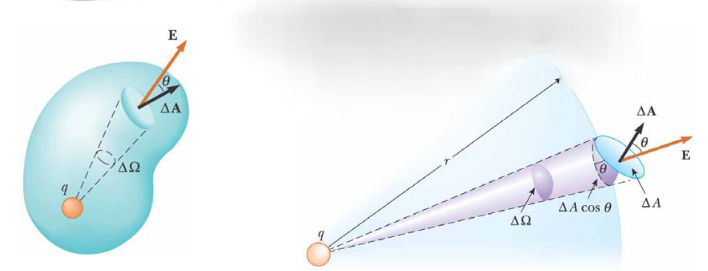
\includegraphics[width=0.7\linewidth]{bewijs_gauss}
		%Blob de vlek%
   		\label{fig:bewijsgauss}
   	\end{figure}
   Eerst legt men de definitie voor de ruimtehoek uit. \textbf{Ruimtehoek} = het oppervlakte van een segment $\Delta A$, geprojecteerd op een eenheidsbol (bol met straal r=1m). Deze wordt uitgedrukt in sterradialen op een analoge wijze als onze gekende radialen. De ruimtehoek wordt als volgt gedefinieerd:
   \[\Delta\Omega = \frac{\Delta A}{r^2} \xrightarrow{\text{volledige sfeer}} \Delta\Omega = \frac{4\pi r^2}{r^2} = 4\pi sterradialen\]
   
   Nu we een manier hebben om een deel van het oppervlak te definieren kunnen we gebruik maken van de verandering in flux.
   \[\Delta\Phi_E = \vec{E}\cdot\Delta\vec{A} = (Ecos\theta)\Delta A\]
   Het elektrisch veld opgewekt door een puntlading wordt als volgt gedefinieerd: \(E = k_eq/r^2\). Hier kan men ook $\Delta A cos\theta$ vervangen door $r^2\cos$ dankzij de definitie van de ruimtehoek. Dit vullen we dan in:
   \[= k_e\frac{q}{r^2}\Delta A cos\theta = k_eq\Delta\Omega\]
   
   Nu we een formule hebben voor de verandering in flux, kan men een totale flux berekenen: 
   \[\Phi_E = k_eq\int \frac{dA\cos\theta}{r^2} = k_eq\int d\Omega = 4\pi k_e q = \frac{q}{\epsilon_0}\]
   
   \textit{Buiten een oppervlak}
   \begin{figure}[h]
   	\centering
   	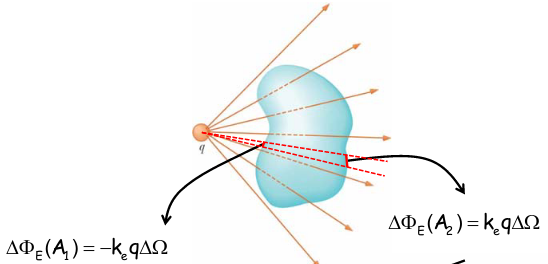
\includegraphics[width=0.7\linewidth]{null.png}
   	\label{fig:nul}
   \end{figure}
	Hier is het belangrijkste al uitgewerkt op de tekening. Je vult de formule voor het verschil in flux in en telt dan al die kleine deeltjes op om de totale flux te bekomen, wat altijd op nul zal uitkomen bij een gesloten oppervlak als de lading zich daar buiten bevind.
   \newline
   
   \textit{Veralgemening:} \(\Phi_E = \int\vec{E}\cdot d\vec{A} = \frac{q_{in}}{\epsilon_0}\)
   	
   	\subsection{Geleider in elektrostatisch evenwicht}
   	Elektrostatisch evenwicht $\iff$ geen netto ladingsbeweging
   	\begin{enumerate}
   		\item Het elektrisch veld in de geleider is nul.
   		Bij een veld verschillend van nul zullen er elektronen bewegen en is er dus geen evenwicht. 
   		\item De lading van een geïsoleerde geleider bevindt zich aan het oppervlak.
   		Het elektrisch veld binnen de geleider is nul, dus ook op het gaussisch oppervlak, dit betekent dat de flux nul is. Er is dus geen nettolading binnen het oppervlak.
   		\item Het elektrisch veld net buiten de geleider : loodrecht op het oppervlak, $\abs{E} = \frac{\sigma}{\epsilon_0}$. 
   		Als dit niet zo zou zijn, zou het elektrisch veld niet loodrecht staan op het oppervlak en zou er een beweging zijn van de elektronen. Dit kan niet gezien het gegeven dus moet het loodrecht staan op het oppervlak.
   		\item Oppervlakteladingsdichtheid is het grootst bij de grootste oppervlaktekromming. 
   	\end{enumerate}
    
    Vergeet bij dit hoofdstuk niet vooral oefeningen te maken en voorbeelden uit het boek! De wet van gauss is vooral praktisch belangrijk!
    \section{Elektrische potentiaal}
    23.1-23.9

    \subsection{Elektrisch Potentiaal}
    In hoofdstuk 7 hebben we arbeid geïntroduceerd. Arbeid kan echter alleen worden gebruikt wanneer
    de kracht die ``arbeid' levert'' conservatief is. We hebben enkele van deze krachten gezien zoals de
    gravitatiekracht en de veerkracht. De elektrische kracht is ook zo'n conservatieve kracht waarvoor
    we arbeid dus kunnen definiëren. Uit hoofdstuk 21 weten we dat de kracht op een testlading in een
    elektrisch veld gegeven is door: 
    
    $$\vec{F} = q_{0} \vec{E}$$
    
    Als we deze lading nu verplaatsen over een afstand $ds$, kunnen we de arbeid berekenen verricht 
    door de elektrische kracht:
    
    $$dW = \vec{F_{e}} \cdot d\vec{s} = q_{0}\vec{E} \cdot d\vec{s}$$
    
    Ook hebben we in hoofdstuk 7 gezien dat $W = -\Delta U$. We kunnen dus de potentiële energie van
    het systeem bepalen:
    
    $$dU = -W$$
    $$\Luda$$
    $$dU = -\vec{F} \cdot d\vec{s}$$
    $$\Luda$$
    $$dU = -q_{0}\vec{E} \cdot d\vec{s}$$
    
    Als we nu de verandering in potentiële energie willen berekenen tussen twee punten A en B, dan vinden 
    we de volgende uitdrukking:
    
    $$\Delta U = U_{b} - U_{a} = -q_{0} \int_{A}^{B} \vec{E} \cdot d\vec{s}$$
    
    We zien dus dat het verschil in potentiële energie niet afhangt van het gevolgde pad, maar alleen van 
    de punten A en B. Een goede opmerking is dat de potentiële energie zal verminderen wanneer de verplaatsing
    in de richting is van de kracht.
    
    We hebben het elektrische veld gedefiniëerd als de kracht per testlading: $\vec{E} = \frac{\vec{F}}{q_{0}}$. 
    We kunnen een analoge denkwijze toepassen op het verschil in potentiële energie:
    
    $$\frac{\Delta U}{q_{0}} = -\int_{A}^{B} \vec{E} \cdot d\vec{s}$$. Deze uitdrukking definiëren we als het
    potentiaalverschil $\Delta V = \frac{\Delta U}{q_{0}}$. Het potentiaal in een punt is dan $V = \frac{U}{q_{0}}$. Let echter goed op! Het potentiaalverschil
    is niet hetzelfde als het verschil in potentiële energie! Potentiaalverschil is namelijk het verschil in potentiële energie
    gedeeld door de testlading $q_{0}$. Aangezien enkel het verschil in potentiële energie fysisch zinvol is, en dus ook
    enkel het potentiaalverschil, moeten we ergens het potentiaal $V = 0$ kiezen. Dit doen we meestal op $\infty$. 
    
    Uit dit potentiaalverschil kunnen we ook rechtstreeks de arbeid berekenen verricht door een externe kracht:
    
    $$W = \Delta U = q\Delta V$$
    
    Het potentiaalverschil wordt uitgedrukt in Volt: 1V = 1J/C.\\
    \\
    Laten we het potentiaalverschil berekenen voor een uniform elektrisch veld:
    
    $$\Delta V = V_{B} - V_{A} = \frac{\Delta U}{q_{0}} = -\int_{A}^{B} \vec{E} \cdot d\vec{s} = -\int_{A}^{B} Eds = -E\int_{A}^{B} ds = -Ed$$
    $$\Delta U = q_{0} \Delta V$$
    
    Een andere goede opmerking is dat de veldlijnen van een elektrisch veld altijd wijzen in de richting van afnemende potentiaal. We kunnen dit gemakkelijk zien
    aan de hand van een voorbeeld. Nemen we een positief en negatief geladen plaat en een positieve testlading aan de positieve plaat. Eens we deze testlading
    loslaten zal deze in de richting van het veld naar de negatieve plaat bewegen (herinner: veldlijnen gaan altijd van positief naar negatief!). Zoals we in 
    hoofdstuk 21 hebben gezien met de wetten van Newton, wint het systeem aan kinetische energie: snelheid. We hebben hier echter alleen verklaart
    waar de kinetische energie vandaan kwam. Volgens de wet van behoud van energie moet deze kinetische energie ergens van komen. Inderdaad,
    de potentiele elektrische energie die de testlading heeft aan de positieve plaat wordt omgezet in deze kinetische energie. Dankzij behoud van energie weten we dan 
    dat de testlading potentiële elektrische energie verliest naarmate het naar de negatieve plaat beweegt en dus dat het potentiaal afneemt in de richting van de 
    veldlijnen. \\
    
    \begin{figure}[h]
    	\centering
	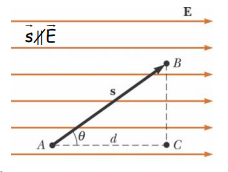
\includegraphics[width=0.4\linewidth]{equipot_oppervlakken}
    	\caption{Equipotentiaaloppervlakken}
        	\label{equipot_opp}
    \end{figure}
    
    Kijken we naar de bijgevoegde figuur, kunnen we zelfs redeneren dat punten B en C dezelfde potentiaal hebben. 
    
    $$\Delta V = -\int_{A}^{B} \vec{E} \cdot d\vec{s} = -\vec{E} \cdot \vec{s}$$
    
    Dit scalair product kunnen we uitwerken als:
    
    $$-\vec{E} \cdot \vec{s} = -Es\cos{\theta}$$
    
    Hierbij substituëren we $cos{\theta}$ met $\cos{\theta} = \frac{d}{s}$ en dus bekomen we:
    
    $$-\vec{E} \cdot \vec{s} = -Es\frac{d}{s} = -Ed$$
    
    Waarbij $-Ed$ het potentiaal is in punt C. Voor een uniform elektrisch veld geldt in het algemeen dat
    alle punten in een vlak loodrecht op het elektrisch veld dezelfde potentiaal hebben. Over het algemeen (niet
    per se uniforme velden) kunnen we zeggen dat een equipotentiaaloppervlak een oppervlak is bestaande uit
    punten met dezelfde elektrische potentiaal.
    
    \subsection{Elektrisch potentiaal/potentiële energie bij puntladingen}
    Herinner dat we het elektrisch veld voor een puntlading hebben berekend: $E = k_{e} \frac{Q}{r^{2}}$. Nu kunnen we
    gemakkelijk het potentiaalverschil berekenen tussen twee punten op straal $r_{a}$ en $r_{b}$ van de puntlading: 
    
    $$\Delta V = V_{b} - V_{a} = -k_{e}Q\int_{r_a}^{r_b} \frac{dr}{r^{2}}$$
    $$\Luda$$
    $$\Delta V = k_{e}Q \left( \frac{1}{r_{b}} - \frac{1}{r_{a}} \right)$$
    
    Hier kiezen we $V = 0$ voor $r_{a} = \infty$ en vinden we dat $V_{b} = \frac{k_{e}Q}{r}$. Als we met
    meerdere puntladingen hebben te maken kunnen we het superpositieprincipe gebruiken, namelijk dat:
    
    $$V = k_{e}\sum_{i} \frac{Q_{i}}{r_{i}}$$

    \subsection{Elektrisch veld afleiden uit de eletrische potentiaal}
    We hebben de hele tijd gewerkt met het feit dat $\Delta V = \frac{\Delta U}{q_{0}} = -\int_{A}^{B} \vec{E} \cdot d\vec{s}$. We nemen
    nu $\Delta V$ infinitisemaal klein:
    
    $$dV = -\vec{E} \cdot d\vec{s}$$
    
    Waaruit de dus kunnen afleiden dat:
    
    \begin{equation}
    	\begin{cases}
      		E_{x} = -\frac{\partial V}{\partial x}\\
      		E_{y} = -\frac{\partial V}{\partial y}\\
      		E_{z} = -\frac{\partial V}{\partial z}\\
    	\end{cases}\,
    \end{equation}
    
    We vinden dus dat: $\vec{E} = -\mathbb{\nabla}{V}$.
    
    \subsection{Elektrische potentiaal van een geladen geleider}
    Voor een geleider in evenwicht geldt dat: $\vec{E} \cdot d\vec{l} = 0$ en dus dat $\Delta V = 0$ (dit kan
    je eenvoudig nagaan door de definitie van potentiaalverschil te gebruiken). We weten dat het oppervlak van een
    geleider in elektrostatisch evenwicht een constante potentiaal heeft. We weten dus ook dat er binnenin de geleider
    een constante potentiaal is! 
    
    We zien dus dat er geen arbeid nodig is om een lading te verplaatsen binnen een geleider, immers: $\Delta U = q\Delta V = 0q = 0$.
    We hebben eerder gezien dat een geleider zich gedraagt alsof de lading allemaal in één punt zit en dus is het elektrisch veld voor een
    geleider:
    
    $$V = k_{e}\frac{Q}{R}$$
    
    We kunnen $Q$ schrijven in termen van de ladingsdichtheid $\sigma$: $Q = \sigma A$ waarbij A het oppervlak is van de geleider. Dan krijgen we:
    
    $$V = k_{e}\frac{\sigma A}{R} = k_{e} \frac{\sigma 4\pi R^{2}}{R} = k_{e}\sigma 4 \pi R$$
    
    Als we twee geleiders nemen met elk hun elektrisch veld is:
    
    $$\frac{E_{1}}{E_{2}} = \frac{\sigma_{1}}{\sigma_{2}} = \frac{R_{1}}{R_{2}}$$ 
    
    waarbij $\sigma = \frac{V}{k_{e}4\pi R}$. We kunnen zien dat het elektrische veld sterker is
    nabij convexe punten!

    \section{Condensatoren en diëlektrica}
    24.2-24.6
    
    \subsection{Condensatoren}
    Een condensator is een instrument om elektrische lading en energie in op te slaan. De bouw van een
    condensator is vrij simpel: Twee geleiders met oppervlakte $A$ op een afstand $d$ van elkaar met
    ertussen een diëlektricum (zie later). Als de condensator geladen is hebben de geleiders dezelfde 
    tegengestelde lading. We kunnen dan de hoeveelheid lading of capaciteit die wordt opgeslagen definiëren als
    de verhouding van de absolute waarde van de elektrische lading op één van de geleiders en het
    potentiaalverschil tussen de geleiders:
    
    $$C = \frac{Q}{\Delta V}$$

    Capaciteit wordt uitgedrukt in Farad: 1F = 1C/V.
    
    \subsection{Berekenen van de capaciteit van een condensator}
    Als we de capaciteit willen kennen moeten we het potentiaalverschil kennen. Dit kunnen
    we berekenen met gebruik van de uitdrukking:
    
    $$\Delta V = -\int_{A}^{B} \vec{E} \cdot d\vec{s}$$
    
    We nemen als voorbeeld een geïsoleerde, geleidende geladen bol met straal $R$ en lading $Q$. Stel dat
    we nu een tweede bol nemen op een afstand $\infty$ van de eerste bol met lading $-Q$. We kunnen het potentiaalverschil
    dan berekenen (potentiaal van een puntlading is berekend in 18.3. Een geleidende geladen bol doet alsof alle lading in één punt zit):
    
    $$\Delta V = V_{r = R} - V_{r = \infty} = k_{e}Q\left(\frac{1}{R}\right) = k_{e}\frac{Q}{R}$$
    $$\Luda$$
    $$C = \frac{Q}{\Delta C} = \frac{Q}{\frac{k_{e}Q}{R}} = \frac{R}{k_{e}} = 4\pi \epsilon_{0} R$$
    
    Als tweede voorbeeld berekenen we de capaciteit van een parallelle-platen condensator. Van parallelle platen weten 
    we dat ze oppervlak $A$ hebben het elektrische veld $E = \frac{\sigma}{\epsilon_{0}}$ waarbij $\sigma = \frac{Q}{A}$.
    Het potentiaalverschil tussen de platen berekenen we als volgt:
    
    $$\Delta V = -\int_{A}^{B} \vec{E} \cdot d\vec{l} = Ed = \frac{\sigma}{\epsilon_{0}}d = \frac{Qd}{\epsilon_{0} A}$$
    
    Dan vinden we voor de capaciteit:
    
    $$C = \frac{Q}{\Delta V} = \frac{Q}{\frac{Qd}{\epsilon_{0} A}} = \epsilon_{0} \frac{A}{d}$$
    
    \subsection{Combinaties van condensatoren}
    We stellen enkele nieuwe symbolen voor:
    
    \begin{enumerate}
    	\item Een condensator: \begin{circuitikz} \draw (0, 0) to[capacitor] (2, 0); \end{circuitikz}
    	\item Een batterij: \begin{circuitikz} \draw (0, 0) to[battery1] (2, 0); \end{circuitikz}
    	\item Een schakelaar: \begin{circuitikz} \draw (0, 0) to[closing switch] (2, 0); \end{circuitikz}
    \end{enumerate}

    We bekijken eerst een parallelle schakeling waarin twee condensatoren rechtstreeks aan de batterij hangen:
    
    \begin{center}
    	\begin{circuitikz}
    		\draw (0, 0)
    		to[battery1, l=$\Delta V$] (2, 0)
    		(0, 0)
    		to[short, *-] (0, 2)
    		(2, 0)
    		to[short, *-] (2, 2)
    		(0, 2)
    		to[capacitor, l=$C_{1}$] (2, 2)
		(0, 2)
		to[short, *-] (0, 4)
		(2, 2)
		to[short, *-] (2, 4)
		(0, 4)
		to[capacitor, l=$C_{2}$] (2, 4);
    	\end{circuitikz}
    \end{center}
    
    Het potentiaalverschil over alle condensatoren is in dit geval hetzelfde, namelijk $\Delta V$. Dan zijn:
    
    \begin{enumerate}
    	\item $Q_{1} = C_{1}\Delta V$
    	\item $Q_{2} = C_{2}\Delta V$
    \end{enumerate}
    
    aangezien $Q = Q_{1} + Q_{2}$. Dus moet $Q = C_{1}\Delta V +  C_{2}\Delta V$. Dan kunnen we een equivalente
    capaciteit beschouwen als: $C_{eq} = C_{1} + C_{2}$ en in het algemeen:
    
    $$C_{eq} = \sum_{i} C_i$$

    We kunnen de stroomkring ook hertekenen als:

    \begin{center}
    	\begin{circuitikz}
    		\draw (0, 0)
    		to[battery1, l=$\Delta V$] (2, 0)
    		(0, 0)
    		to[short, *-] (0, 4)
    		(2, 0)
    		to[short, *-] (2, 4)
    		(0, 4)
    		to[capacitor, l=$C_{eq}$] (2, 4);
    	\end{circuitikz}
    \end{center}

    We bekijken nu een serieschakeling:
    
    \begin{center}
    	\begin{circuitikz}
    		\draw (0, 0)
    		to[battery1, l=$\Delta V$] (4, 0)
    		to[short, *-] (4, 2)
    		to[capacitor, l=$C_{2}$] (3, 2)
    		to[short, *-] (1, 2)
    		to[capacitor, l=$C_{1}$] (0, 2)
    		to[short, *-] (0, 0);
    	\end{circuitikz}
    \end{center}
    
    Nu is niet het potentiaalverschil maar de lading gelijk over alle condensatoren, namelijk $Q$. Dan zijn:
    
    \begin{enumerate}
    	\item $\Delta V_{1} = \frac{Q}{C_{1}}$
    	\item $\Delta V_{2} = \frac{Q}{C_{2}}$
    \end{enumerate}

    aangezien $\Delta V = \Delta V_{1} + \Delta V_{2}$. Dus moet $\Delta V = \frac{Q}{C_{1}} + \frac{Q}{C_{2}}$. Dan kunnen we een
    equivalente capaciteit beschouwen als: $\frac{1}{C_{eq}} = \frac{1}{C_{1}} + \frac{1}{C_{2}}$ en in het algemeen:
    
    $$C_{eq} = \sum_{i} \frac{1}{C_{i}}$$
    
    We kunnen de stroomkring ook hertekenen als:
    
     \begin{center}
    	\begin{circuitikz}
    		\draw (0, 0)
    		to[battery1, l=$\Delta V$] (4, 0)
    		to[short, *-] (4, 2)
    		to[capacitor, l=$C_{eq}$] (0, 2)
    		to[short, *-] (0, 0);
    	\end{circuitikz}
    \end{center}
    
    \subsection{Energie opgeslagen in een geladen condensator}
    In een condensator wordt er lading overgebracht van de negatieve naar de positieve pool. Initieel is er geen arbeid nodig om een kleine
    hoeveelheid lading $dq$ te verplaatsen (aangezien de lading op de positieve plaat 0 is, en er dus nog geen krachten inwerken op $dq$). 
    
    Eens dat $dq$ wel verplaatst is, zal er wel arbeid nodig zijn om een nieuwe $dq$ te verplaatsen, aangezien de eerste ladingstransfert ervoor
    heeft gezorgd dat er zich nu een potentiaalverschil bevindt tussen te positieve en de negatieve plaat. Hoe meer lading er wordt overgezet,
    hoe meer arbeid er dus nodig zal zijn om een nieuw stukje lading over te zetten.
    
    Stel er bevindt zich een lading $q$ op de positieve plaat, dan is $\Delta V = \frac{q}{C}$ en dan is $dW = \Delta V dq = \frac{q}{C}dq$. We
    kunnen nu dus de arbeid berekenen om een infinitisemale lading $dq$ over te zetten van de positieve naar de negatieve plaat wanneer er zich reeds
    een lading $q$ op de positieve plaat bevindt:
    
    $$W = \int_{0}^{Q} \frac{q}{C}dq = \frac{1}{C} \int_{0}^{Q}qdq = \frac{Q^{2}}{2C}$$
    
    Dan vinden we dat $U = \frac{Q^{2}}{2C} = \frac{Q\Delta V}{2} = \frac{C(\Delta V)^{2}}{2}$
    We definiëren ook een energiedichtheid tussen de oppervlakken van de condensator:
    
    $$U_{e} = \frac{\epsilon_{0}E^{2}}{2}$$
    
    Deze uitdrukking is geldig voor eender welk elektrisch veld.
    
    \subsection{Condensatoren met een diëlektricum}
    We hebben gezegd dat de zicht in de ruimte $d$ tussen de oppervlakken van de condensator zich een diëlektricum
    bevindt. Dit diëlektricum is een isolator die de capaciteit van de condensator verhoogt met een factor $\kappa$:
    
    $$C_{0} = \frac{Q_{0}}{\Delta V_{0}} < C = \frac{Q_{0}}{\Delta V} \textit{ met } C = \kappa C_{0}$$
    
    Het diëlektricum zorgt voor een afname in potentiaalverschil, en dus een toename in capaciteit. We dus beredeneren 
    dat een diëlektricum het elektrische veld van een ladingsverdeling afzwak. 
    

    \section{Elektrische stroom en weerstand}
    25.1-25.6, 25.8-25.9 (+40.7-40.10)
    \subsection{De wet van Ohm}
    De stroom doorheen een draad is recht evenredig met het potentiaalverschil over de twee uiteinden.
    \[V = IR\]
    
    \subsection{Resistiviteit}
    Hetgeen dat volgt is experimenteel vastgelegd:
    De weerstandR van een draag is 1) recht evenredig met de lengte l van de weerstand en 2) omgekeerd evenredig met de doorsnede A.
    \[R = \rho\frac{l}{A}\]
    met $\rho$ de resistiviteit van de geleider. Deze is afhankelijk van het materiaal en van de temperatuur. Voor deze laatste is er ook een formule: 
    \[\rho = \rho_0[1 + \alpha (T - T_0)]\]
    
    \subsection{Elektrische energie en vermogen}
    Er is een energietransfer van de batterij naar het 'toestel', er zal in het toestel dus een energieverlies zijn. 
    
    We hebben hier al een uitdrukking voor gezien, namelijk Vermogen: 
    \[P = \frac{dU}{dt} = \frac{d}{dt}(q\Delta V) = \frac{dq}{dt}\Delta V = I\Delta V\]
    
    Het elektrisch vermogen wordt dus als volgt gedefinieerd: 
    \[P = I\Delta V = I^2R = \frac{(\Delta V)^2}{R}\]
    De eenheid hiervoor is Watt.
    
    \subsection{Microscopisch model van elektrische stroom}
    Wanneer er een spanning wordt geplaatst op de batterij, zal er een elektrisch veld ontstaan dat evenwijdig is met de wanden van de draad. Dit gaat er dus voor zorgen dat er elektronen zullen bewegen in de draag. We kunnen vanuit de stroom een gemiddelde stroom bepalen: 
    
    \[I_{gem} : \frac{\Delta Q}{\Delta t} = nqv_dA\]
    Waarbij n aantal lading in dat deel, q de lading, $v_d$ de driftsnelheid van de elektronen. De driftsnelheid is de snelheid van de elektronen op een rechte schaal, deze bewegen volledig random door een materiaal maar wij hebben hun snelheid nodig tegenover de x-as. Lading wordt hier dan gedefinieerd door \((nA\Delta x)q\) met \(\Delta x = v_d \Delta t\)
    
    Met hetgeen we nu hebben gevonden kunnen we de stroomdichtheid definiëren. Dit is dus stroom per oppervlakte (van de draad). 
    
    \[j = \frac{I}{A} : nqv_d\]
    
    \subsection{Microscopisch model van elektrische stroom}
    Nu we stroomdichtheid hebben kunnen definiëren, kan men hieruit de echt wet van Ohm afleiden. \(\vec{J} = nq\vec{v}_d\)
    \textit{Wanneer het potentiaalverschil over een geleider constant gehouden wordt, ontstaan een stroomdichtheid J en een elektrisch veld E.}
    \[\vec{J} = \sigma\vec{E}\]
    met $\sigma$ de geleidbaarheid van het materiaal. Dit is gelijk aan $\sigma = 1/\rho$
    
    \textit{Wet van Ohm (de echte): De verhouding van de stroomdichtheid en het elektrisch veld is een constante.}
    
    \textbf{In de praktijk}
    Het potentiaalverschil kan als volgt worden bepaald: \(\Delta V = V_b - V_a = -\int_a^b \vec{E}\cdot d\vec{s} = -E\int_0^ldx = El\).
    We kunnen dus E vervangen in volgende vergelijking en verderwerken tot we de gewone wet van Ohm verkrijgen.
    \[J = \sigma E = \sigma\frac{\Delta V}{l}\]
    \[\Delta V = \frac{l}{\sigma}J = \frac{l}{\sigma A}I = RI\]    
    
    Dit toont dus aan dat de twee 'wetten van Ohm' eigenlijk evenredig zijn. We kunnen door onze kennis over resistiviteit en geleidbaarheid. \[R = \frac{l}{\sigma A} = \rho\frac{l}{A}\]
    
    \subsection{microscopisch model voor elektrische geleiding}
    Leer dit goed! hij heeft het (tot nu) nog niet op een examen gevraagd dus is de kans wel wat groter dat dat eens gaat gebeuren. Dit is een deel dat niet in het boek te vinden is dus luister hier goed naar bij de les.


    \section{Gelijkstroomschakelingen}
    26.2-26.5, 26.7
    
    \subsection{Gelijkstroomkringen}
    Schakelingen met een spanningsbron, weerstand en condensatoren. We mogen in deze gevallen veronderstellen dat de stroom constant is in richting en zin: \textit{Gelijkstroom (DC)}.
    
    \textbf{Elektromotorische "kracht" (emf)}
    De emf $\Epsilon$ is de maximale spanning (of het maximaal potentiaalverschil) dat een batterij kan leveren in de ideale omstandigheden. In werkelijkheid heeft de batterij ook intern een weerstand r, je kan dit ook in de onderstaande figuur zien.
   
    \begin{center}
    	\begin{circuitikz}
    		\draw (0,0)
    		to[battery1, l=$\Epsilon$] (2, 0)
    		to[american resistor, l=$r$] (4, 0);
    	\end{circuitikz}
    \end{center}
	Door deze interne weerstand zal men dus nooit de maximale spanning $\Epsilon$ kunnen benuttigen. De \textit{klemspanning} van de batterij zal dus \(\Delta V_{ab} = V_b - V_a = \Epsilon - Ir\). Hier kan men dus zien dat de spanning stroomafhankelijk zal zijn en wanneer er geen stroom vloeit, de spanning gelijk zal zijn aan $\Epsilon$.
	
	We kunnen ook rekening houden met de weerstand buiten de batterij met volgende formules:
	\[\Epsilon = IR + Ir \Rightarrow I = \frac{\Epsilon}{R + r}\]
	
	We kunnen met deze kennis ook het vermogen van de batterij berekenen:
	\[I\Epsilon = I^2R + I^2r\]
	
	\subsection{Weerstanden in serie en parallel}
	\begin{itemize}
	\item \textbf{Serieschakeling}
    \begin{center}
    	\begin{circuitikz}
    		\draw (0,0)
    		to[battery1, l=$\epsilon$] (8, 0)
    		to[short, *-] (8, 3)
    		to[american resistor, l=$R_{2}$] (4, 3)
    		to[american resistor, l=$R_{1}$] (0, 3)
    		to[short, *-] (0, 0);
    	\end{circuitikz}
    \end{center}
	Alle lading passeert langs elke weerstand, dus in serie zal er \textit{gelijke stroom zijn in alle weerstanden.}
	Het potentiaalverschil van de batterij wordt dus verdeeld over de weerstanden: 
	\[\Delta = IR_1 + IR_2 = I(R_1+R_2) = IR_{eq} \Rightarrow R_{eq} = \sum_i R_i\] 
	
	\item \textbf{Parallelschakeling}
    \begin{center}
    	\begin{circuitikz}
    		\draw (0,0)
    		to[battery1, l=$\epsilon$] (8, 0)
    		to[short, *-] (8, 3)
    		to[short, *-] (6, 3)
    		to[short, *-] (6, 4)
    		to[american resistor, l=$R_{1}$] (2, 4)
    		to[short, *-] (2, 3)
    		to[short, *-] (0, 3)
    		to[short, *-] (0, 0)
    		(6, 3)
    	 	to[short, *-] (6, 2)
    	 	to[american resistor, l=$R_{2}$] (2, 2)
    	 	to[short, *-] (2, 3);
    	\end{circuitikz}
    \end{center}
    De lading wordt verdeeld over beide weerstanden: \(I = I_1 + I_2\). Bij parallelijk zal er \textit{gelijk potentiaalverschil zijn over alle weerstanden.} \[I = I_1+I_2 = \frac{\Delta V}{R_1}+\frac{\Delta V}{R_2} = \Delta V(\frac{1}{R_1} + \frac{1}{R_2}) = \frac{\Delta V}{R_{eq}} \Rightarrow \frac{1}{R_{eq}} = \sum_i \frac{1}{R_i}\]
    
    Er zijn ook verschillende voordelen aan parallelschakeling: Eerste en vooral is de weerstand over alle gebruikers dus kleiner. Als tweede is het feit dat wanneer een lamp (of weerstand) breekt, de rest wel zal blijven werken. Het is in deze situatie dan ook heel gemakkelijk om de kapotte lamp te localiseren en dan te maken. Als laatste zal de stroom door de weerstanden niet worden veranderd als er een weerstand wordt toegevoegd.
	\end{itemize}
	
	\subsection{De regels van Kirchhoff}
	\begin{itemize}
		\item \textbf{\emph{Eerste regel van Kirchhof}}
		\textit{Behoud van lading}: De som van de stromen die een vertakking binnenkomen, moet gelijk zijn aan de som van de stromen die de vertakking verlaten.
		\[\sum I_{in} = \sum I_{uit}\]
		
		\item \textbf{\emph{Tweede regel van Kirchhof}}
		\textit{Behoud van energie}: De som van de potentiaalverschillen over alle elementen in een gesloten kring, moet nul zijn.
		\[\sum_{gesloten kring} \Delta V = 0\]
		Bij deze regel zijn de volgende 'regeltjes' handig te onthouden: 
		\begin{itemize}
			\renewcommand\labelitemi{--}
			\item Weerstand mee met de stroom: \(\Delta V = -IR\)
			\item Weerstand tegen de stroom in: \(\Delta V = +IR\)
			\item emf-bron van - naar + : \(\Delta V = +\Epsilon\)
			\item emf-bron van + naar - : \(\Delta V = -\Epsilon\)
		\end{itemize}
	\end{itemize}
	Deze regels leer je het best door voorbeelden zelf te maken en de oefenzittingen te maken! Dan zullen de regels heel logisch zijn.
	
	\subsection{RC-kringen}
	Een RC-kring ziet er als volgt uit:    
    \begin{center}
    	\begin{circuitikz}
    		\draw (0,0)
    		to[battery1, l=$\epsilon$] (4, 0)
    		to[closing switch, l=$S$] (8, 0)
    		to[short, *-] (8, 3)
    		to[american resistor, l=$R$] (0, 3)
    		to[capacitor, l=$C$] (0, 0);
    	\end{circuitikz}
    \end{center}
	Als men hier de tweede regel van Kirchhof toepassen, krijgen we \(\Epsilon - \frac{q}{c} - IR = 0\). I en q zullen variëren met de tijd. 
	
	Op \emph{t = 0} zal er nog geen lading zijn: \[\Epsilon - I_0R = 0 \rightarrow I_0 = \frac{\Epsilon}{R}\]
	Hier is de condensator nog niet van belang aangezien hier nog helemaal een lading op staat, dus geldt de wet van Ohm gewoon.
	
	Op \emph{t = $\inf$} zal er geen stroom meer zijn: \[\Epsilon - \frac{Q}{C} = 0 \rightarrow Q = C\Epsilon\]
	In dit geval gaat het lijken alsof er geen weerstand is, aangezien er geen stroom is en de weerstand dus geen effect heeft. 
	
	\textbf{Tijdsafhankelijke oplossing}: We zoeken een formule om afhankelijk van de tijd, de stroom en de lading te kunnen bepalen, hiervoor maken we volgende afleiding:
	\[\Epsilon - \frac{q}{C} - IR = 0 \text{  en  } I = \frac{dq}{dt} \rightarrow \frac{dq}{dt} = \frac{\Epsilon}{R} - \frac{q}{RC}\]
	Hierboven hebben we dus de tweede regel van Kirchhof gebruikt om dan nog de stroom I te vervangen door de definite die we ervoor al kennen en dan beide leden door R te delen. We kunnen die laatste vergelijking dan verder herwerken om daarna te kunnen integreren.
	
	\[\frac{dq}{dt} = \frac{C\Epsilon}{RC} - \frac{q}{RC} = -\frac{q - C\Epsilon}{RC} \rightarrow \frac{dq}{q - C\Epsilon} = -\frac{1}{RC}dt\]
	
	We integreren dit van tijd 0 tot t:
	\[\int_0^q \frac{dq}{q-C\Epsilon} = -\frac{1}{RC}\int_0^tdt \rightarrow ln(1-\frac{q}{C\Epsilon}) = -\frac{t}{RC} \rightarrow 1-\frac{q}{C\Epsilon} = e^{-\frac{t}{RC}}\]
	
	En deze hele afleiding geeft dus als formules:
	\[q = C\Epsilon(1 - e^{-\frac{t}{RC}}) = Q(1-e^{-\frac{t}{RC}})\]
	\[I = \frac{dq}{dt} = \frac{\Epsilon}{R}e^{-\frac{t}{RC}}\]
	Hier is de tijdsconstante $\tau = RC$.
	
	\textbf{Energiebalans van de RC-kring}: Hoeveel energie heeft de emf geleverd?
	\[\int_0^{U_{emf}}dU = \int_0^Q\Epsilon dq = \Epsilon\int_0^Qdq \Rightarrow U_{emf} = Q\Epsilon = \Epsilon^2C\]
	
	De energie is eerlijk verdeeld over de condensator en de weerstand:
	\[U_C = U_R = \frac{\Epsilon^2C}{2} \Rightarrow U_{emf} = U_C + U_R\]
    
    \textbf{Ontladen van de condensator}: We gaan zien wat er gebeurt als we de schakelaar openen en de condensator ontlaadt. 
    \begin{center}
    	\begin{circuitikz}
    		\draw (0,0)
    		to[short, *-] (8, 0)
    		to[american resistor, *-] (8, 3)
    		to[short, l=$R$] (0, 3)
    		to[capacitor, l=$C$] (0, 0);
    	\end{circuitikz}
    \end{center}

	\[-\frac{q}{C} - IR = 0 \text{  en  } I = \frac{dq}{dt} \rightarrow -R\frac{dq}{dt} = \frac{q}{C} \rightarrow \frac{dq}{q} = -\frac{1}{RC}dt\]    
	Dit laatste kan men dan weer integreren:
	\[\int_Q^q\frac{dq}{q} = -\frac{1}{RC}\int_0^tdt \rightarrow ln(\frac{q}{Q}) = -\frac{t}{RC} \Rightarrow q = Qe^{-\frac{t}{RC}}\]
	\[I = \frac{dq}{dt} = \frac{d}{dt}(Qe^{-\frac{t}{RC}}) = -\frac{Q}{RC}e^{-\frac{t}{RC}} \Rightarrow -I_0 e^{-\frac{t}{RC}}\]
	Met dezelfde tijdsconstante $\tau = RC$
	
	\textbf{energiebalans van de RC-keten}
	\[\int_{0}^{U_R }dU = \int_{0}^{\infty}Pdt = \int_{0}^{\infty} I^2Rdt = \frac{Q^2R}{R^2C^2}\int_0^\infty e^{\frac{-2t}{RC}}dt = \frac{Q^2RC}{RC^2} = \frac{Q^2}{2C} = U_R = U_C\]
  
    \section{Pollevs}
    \begin{itemize}
    \renewcommand\labelitemi{--}
    \item Drie voorwerpen worden dicht bij elkaar gebracht, twee per twee. Wanneer voorwerp A en B bij elkaar gebracht worden, stoten ze elkaar af. Wanneer voorwerpen B en C bij elkaar gebracht worden, stoten ze elkaar ook af. Hieruit kunnen we besluiten dat:
    \begin{enumerate}[label=\alph*]
    	\item A en C hebben een lading van hetzelfde teken.
    	\item A en C hebben een lading van het tegengestelde teken.
    	\item De drie voorwerpen hebben een lading van hetzelfde teken. 
    	\item Een van de voorwerpen is neutraal. 
    	\item We moeten bijkomende experimenten doen om het teken van de lading te kennen. 
    \end{enumerate}
	\textit{Oplossing}: Eigenlijk zijn er 3 juiste antwoorden. A, C en E. Dit laatste is omdat er technisch gezien bijkomende proeven gedaan moeten worden om te weten welke ladingen het zijn. 
	\newline
	\item Drie voorwerpen worden dicht bij elkaar gebracht, twee per twee. Wanneer voorwerp A en B bij elkaar gebracht worden, trekken ze elkaar aan. Wanneer voorwerpen B en C bij elkaar gebracht worden, stoten ze elkaar af. Hieruit kunnen we besluiten dat: 
	\begin{enumerate}[label=\alph*]
		\item A en C hebben een lading van hetzelfde teken. 
		\item A en C hebben een lading van het tegengestelde teken. 
		\item De drie voorwerpen hebben een lading van hetzelfde teken. 
		\item Een van de voorwerpen is neutraal. 
		\item We moeten bijkomende experimenten doen om het teken van de lading te kennen; 
	\end{enumerate}
	\textit{Oplossing:} Het laatste antwoord is het juiste. Ofwel zullen ze elkaar afstoten, dan is de lading altijd gelijk. Als ze elkaar aantrekken kan dit via aantrekking zijn of door middel van inductie. Bij dit tweede zou A neutraal kunnen zijn. 
	\item Een testlading van +3$\mu$C bevindt zich in een punt P waar er een uitwendig elektrisch veld is (naar rechts gericht) met grootte \(4 \times 10^6 N/C\). Wanneer de testlading vervangen wordt door een andere testlading van -3$\mu$C, zal het elektrsische vel in P
	\begin{enumerate}[label=\alph*]
		\item Onveranderd zijn
		\item Omkeren van richting
		\item Veranderen op een manier die we niet kunnen bepalen. 
	\end{enumerate}
	\textit{Oplossing:} a is het antwoord. Het elektrische veld is onafhankelijk van de (positieve) testlading. Enkel de kracht zal veranderen. 
	\item Veronderstel dat de straal van een sfeer (met straal van 1.00m en een lading van 1$\mu$C in het middelpunt) veranderd wordt naar 0.50m. Wat gebeurt er met de flux door de sfeer en met de grootte van het elektrisch veld op het sfeeroppervlak. 
	\begin{enumerate}[label=\alph*]
		\item De flux en het veld nemen toe.
		\item De flux en het veld nemen af. 
		\item De flux neemt toe, het veld neemt af. 
		\item De flux neemt af, het veld neemt toe. 
		\item De flux blijft constant, het veld neemt toe.
		\item De flux neemt af, het veld blijft constant.
	\end{enumerate}
	\textit{Oplossing:} Het veranderen van de straal verandert niets aan het aantal veldlijnen door het oppervlak van de sfeer. 
	\item Wanneer de nettoflux doorheen een gaussisch oppervlak nul is, kunnen deze drie bewerkingen correct zijn. Welke beweringen moeten corrrect zijn?
	\begin{enumerate}[label=\alph*]
		\item Binnen het oppervlak bevinden zich geen ladingen.
		\item Het elektrisch veld is gelijk aan nul over het ganse oppervlak.
		\item Het aantal veldlijnen die het oppervlak binnen komen, is gelijk aan het aantal veldlijnen die het oppervlak verlaten. 
	\end{enumerate}
	\textit{Oplossing:} Het laatste antwoord is juist. Een tegenvoorbeeld van de twee andere is een ingesloten dipool. 
	\item Een negatieve lading wordt in punt A geplaatst en vervolgens naar punt B gebracht. De verandering in potentiële energie van dit 'lading-veld'-systeem is
	\begin{enumerate}[label=\alph*]
		\item Positief.
		\item Negatief.
		\item Nul.
	\end{enumerate}
	\textit{Oplossing:} Het antwoord is a. \(F = q\vec{E}\). De kracht in een andere zin tov het veld, de lading zal niet vanzelf gebeuren. Een externe kracht moet zorgen voor de verplaatsing, de arbeid geleverd door het elektrische veld is negatief.
	\item De aangeduide punten in de figuur bevinden zich op een reeks equipotentiaaloppervlakken. Rangschik, van groot naar klein, de arbeid verricht door het elektrisch veld op een positief geladen deeltje dat beweegt op de volgende manier: (zie figuur in slides)
	\begin{enumerate}[label=\alph*]
		\item B $\rightarrow$ C, C $\rightarrow$ D, D $\rightarrow$ E, A $\rightarrow$ B
		\item A $\rightarrow$ B, D $\rightarrow$ E, B $\rightarrow$ C, C $\rightarrow$ D
		\item B $\rightarrow$ C, C $\rightarrow$ D, A $\rightarrow$ B, D $\rightarrow$ E
		\item D $\rightarrow$ E, A $\rightarrow$ B, C $\rightarrow$ D, B $\rightarrow$ C
	\end{enumerate}
	\textit{Oplossing:} c is het juiste antwoord. \(q_0 \delta = -W_e\) waarbij $q_0$ een positieve lading is. Dat betekend dus dat de arbeid gelijk is aan het negatieve van de verandering in potentiaal. Dan is B $\rightarrow$ C = 2, C $\rightarrow$ D = 1, A $\rightarrow$ B = 0, D $\rightarrow$ E = -1.
	\item Als de potentiaal in functie van de plaats gegeven wordt door de links figuur (zie slides), hoe ziet het elektrisch veld in functie van de plaats er dan uit?
	\begin{enumerate}[label=\alph*]
		\item A
		\item B
		\item C
		\item D
	\end{enumerate}
	\textit{Oplossing:} Het juiste antwoord is b. Dit kan gemakkelijk gevonden worden door de grafiek af te leiden volgens volgende formule: \(E_x = -\frac{dV}{dx}\). Het deel dat discontinu is zal bij het afleiden gewoon oneindig vormen (wegen delen door 0).
	\item Een condensator bezit een lading Q bij een potentiaalverschil $\Delta$V. Wanneer de batterijspanning verdubbeld wordt naar 2$\Delta$V, dan:
	\begin{enumerate}[label=\alph*]
		\item halveert de capaciteit en blijft de lading gelijk
		\item halveren zowel de capaciteit als de lading
		\item verdubbelen zowel de capaciteit als de lading
		\item blijft de capaciteit gelijk en verdubbelt de lading
	\end{enumerate}
	\textit{Oplossing:} D is hier het juiste antwoord. De lading is afhankelijk van potentiaalverschil, de capaciteit blijft altijd constant wanneer de fysische eigenschappen niet veranderen.
	\item De meeste toetsenbordknoppen bevatten een condensator. Wanneer de toets ingedrukt wordt, wordt de zachte isolator tussen de beweegbare en de vaste plaat samengedrukt. Hierbij zal de capaciteit
	\begin{enumerate}[label=\alph*]
		\item Stijgen
		\item Dalen
		\item veranderen op een manier die we niet kunnen voorspellen omdat het elektronisch circuit de spanning over de toets kan veranderen. 
	\end{enumerate}
	\textit{Oplossing:} Het juiste antwoord is A. Kijk hiervoor naar de formule met de afhankelijkheid tussen de capaciteit en de afstand tussen de twee platen. C is fout omdat de capacteit met deze formule niet afhangt van de lading. 
	\item Twee condensatoren zijn identiek. Ze kunnen in serie of in parallel geschakeld worden. Om de \textit{kleinste} equivalente capaciteit te bekomen, moet je ze schakelen in
	\begin{enumerate}[label=\alph*]
		\item serie
		\item parallel
		\item beide resulteren in dezelfde capaciteit
	\end{enumerate}
	\textit{Oplossing:} A is het juiste. Bij parallel stijgt de capaciteit en bij serie daalt die. Simpel voorbeeld: stel $C_1 = 2 = C_2$, dan is voor parallel \(C_{tot} = 2 + 2 = 4\) en voor serie \(1/C_{tot} = 1/2 + 1/2 = 1\)
	\item Twee condensatoren zijn identiek. Elke condensator wordt opgeladen tot een spanning van 10V. Om het grootste gecombineerde potentiaalverschil te bekomen, moet je ze schakelen in
	\begin{enumerate}[label=\alph*]
		\item serie
		\item parallel
		\item beide resulteren in hetzelfde potentiaalverschil
	\end{enumerate}
	\textit{Oplossing:} A is de juiste oplossing. Bij serie zal men alle potentiaalverschillen optellen en zal dus 20V uitkomen, terwijl die bij parallel gewoon 10V blijft. 
	\item Je hebt drie condensatoren en een batterij ter beschikking. In welke condensatorschakeling zal je de maximale hoeveelheid energie opslaan?
	\begin{enumerate}[label=\alph*]
		\item Serie
		\item Parallel
		\item Beide schakelingen zullen evenveel energie opslaan.
	\end{enumerate}
	\textit{Oplossing}: B is het juiste antwoord. We kijken hiervoor naar \(U = C(\Delta V)^2 / 2\). Bij een parallele schakeling moeten de spanningen gewoon opgeteld worden en dit zal dus voor meer energie zorgen tegenover een parallele schakeling.
	\item Je laadt een parallelle-platencondensator op, ontkoppelt die vervolgens van de batterij en zorgt ervoor dat de platen elkaar niet raken. 
	
	Wanneer je de platen \textit{verder uit elkaar trekt}, zullen de volgende grootheden dan toenemen, afnemen of gelijk blijven? 
	\begin{enumerate}[label=\alph*]
		\item C
		\item Q
		\item E tussen de platen
		\item $\Delta$V
		\item Opgeslagen energie in de capacitor
	\end{enumerate} 
	\textit{Oplossing}: De oplossing met de uitleg wordt per grootheid gegeven. 
	\begin{enumerate}[label=\alph*]
		\item C zal afnemen, dit kan je gemakkelijk zien in volgende formule: \(C_{||} = \epsilon_0 \frac{A}{d}\)
		\item Q zal gelijk blijven, er kan geen lading bijkomen of weggaan aangezien de batterij ontkoppeld is.
		\item Het elektrisch veld zal ook gelijk blijven aangezien enkel de lading van belang is en deze ook gelijk blijft. 
		\item Het potentiaalverschil zal toenemen, dit kan je op twee manieren zien: \(\Delta V = Ed \rightarrow\) E blijft gelijk $\rightarrow$ d zal stijgen en dus zal $\Delta$V ook stijgen. De andere manier is: \(C = \frac{Q}{\Delta V} \rightarrow\) C zal dalen zoals we bij a zagen en lading blijft gelijk $\rightarrow$ $\Delta$V stijgt.
		\item De energie zal ook stijgen. Deze energie zal komen uit de arbeid die geleverd moet worden om de platen uit elkaar te trekken, het tegenwerken van de aantrekkingskracht. Je kan dit ook zien met behulp van de volgende formules: \(U = \frac{Q^2}{2C} = \frac{C()\Delta V)^2}{2} = \frac{Q\Delta V}{2}\)
	\end{enumerate}
	\item If you have ever tried to hand a picture or a mirror, you know it can be difficult to locate a wooden stud in which to anchor you nail or screw. A carpenter's stud-finder is basically a capacitor with its plates arranged side by side instead of facing one another, as shown in the figure (zie slides). When the device is moved over a stud, the capacitance will:
	\begin{enumerate}[label=\alph*]
		\item increase
		\item decrease
	\end{enumerate}
	\textit{Oplossing}: De diëlektrische constante van hout zal hoger liggen dan die van de lucht, dus zal de capaciteit stijgen. 
	\item Een volledig opgeladen parallelle-platencondensator blijft aan de batterij verbonden terwijl je een diëlektricum tussen de platen inbrengt. Zal de volgend grootheid toenemen, afnemen of gelijk blijven?
	\begin{enumerate}[label= \alph*]
		\item C
		\item Q
		\item E tussen de platen
		\item $\Delta$V
	\end{enumerate}
TODO: LES HERBEKIJKEN VOOR BETERE UITLEG
	\textit{Oplossing}:
	\begin{enumerate}[label=\alph*]
		\item De capaciteit zal toenemen. 
		\item De lading zal toenemen. 
		\item Het elektrisch veld tussen de platen zal gelijkblijven. 
		\item Het potentiaalverschil zal gelijk blijven, die kan men zien door volgende formule: \(E = \frac{\Delta}{d}\).
	\end{enumerate}
	De energie zal stijgen bij het wegnemen van het diëlektricum. 
	\item Positieve en negatieve ladingen bewegen horizontaal doorheen de vier gebieden in de figuur (zie slides). Rangschik de grootte van de stroom, van klein naar groot. 
	\begin{enumerate}[label=\alph*]
		\item a, b, c
		\item b, c, a
		\item c, d, a
		\item d, b, a
	\end{enumerate}
	\textit{Oplossing}: Het juiste antwoord zal D zijn. We hebben de conventionele stroomzin bepaalt mbv de positieve lading. Dit betekent dat wanneer de negatieve lading in de tegengestelde richting beweegt (tov de positieve lading) deze bijdraagt aan de stroomzin en dus bij kan worden geteld bij de lading. In elke tekening mogen we de ladingen dus gewoon bij elkaar optellen en zo weten we waar de grootste stroom is. Een andere uitleg is dat de positieve ladingen naar rechts bewegen en dus wordt de linkerkant van de draad negatiever met de tijd. Dit is ook het geval met de negatieve ladingen die naar links bewegen. Ze bouwen dus op elkaar op. 
	\item Je laat de spanning over een gloeilamp gradueel toenemen, terwijl je de stroom meet. Bovendien ondervind je dat de temperatuur van de lamp toeneemt naarmate de spanning stijgt. Welke curve geeft jouw experimentele data best weer? (zie slides voor figuren).
	\begin{enumerate}[label=\alph*]
		\item 
		\item 
		\item 
		\item 
	\end{enumerate}
	\textit{Oplossing}: De Helling van de I-$\Delta$V grafiek is 1/R. De weerstand zal hier duidelijk stijgen en dus zal de grafiek moeten dalen. c is de enige dalende grafiek. 
	\item Hetzelfde potentiaalverschil wordt aangelegd over beide lampen. Welke uitrukking klopt? (Er is een afbeelding van een 30-W lamp en een 60-W lamp).
	\begin{enumerate}[label=\alph*]
		\item De 30-W lamp heeft de hoogste stroom en de hoogste weerstand. 
		\item De 30-W lamp heeft de hoogste stroom maar de 60-W lamp heeft de hoogste weerstand.
		\item De 30-W lamp heeft de hoogste weerstand maar de 60-W lamp heeft de hoogste stroom. 
		\item De 60-W lamp heeft de hoogste stroom en de hoogste weerstand. 
	\end{enumerate}
	\textit{Oplossing}: c is hier het juiste antwoord. We beginnen bij \(R = \frac{(\Delta V)^2}{P}\). Als we hier P al eens invullen zien we dat de weerstand zal stijgen bij de 30-W lamp en zal dalen bij de 60-W lamp. Voor stroom kunnen we dan kijken naar de afgeleide wet van Ohm: \(R = \frac{\Delta V}{I}\). De weerstand zal bij 30-W stijgen, dus zal de stroom moeten dalen zodat de spanning constant blijft. Met deze denkwijze komt men te weten dat de stroom zal stijgen bij de 60-W lamp. 
	\item Een stroomvoerende Ohmse draad heeft een diameter die geleidelijk kleiner wordt van links naar rechts. Omdat de stroom overl even groot moet zijn (zodat de lading nergens accumuleert), zullen de driftsnelheid en de weerstand;
	\begin{enumerate}[label=\alph*]
		\item Beide toenemen
		\item Beide afnemen
		\item De driftsnelheid neemt toe en de weerstand neemt af
		\item De driftsnelheid neemt af en de weerstand neemt toe
	\end{enumerate}
	\textit{Oplossing}: Ze zullen beide toenemen. De weerstand zal toenemen doordat: \(R = \rho\frac{l}{A} \rightarrow A\downarrow \rightarrow R\uparrow\). De driftsnelheid zal ook toenemen: \(I = nqv_dA \rightarrow A\downarrow \rightarrow v_d\uparrow\) en dit doordat de stroom gelijk blijft. 
	\item Om de fractie van het vermogen dat door een batterij aan een toestel geleverd wordt, te maximaliseren, moet de inwendige weerstand van de batterij
	\begin{enumerate}[label=\alph*]
		\item Zo laag mogelijk
		\item Zo hoog mogelijk
		\item De fractie hangt niet af van de inwendige weerstand.
	\end{enumerate}
	\textit{Oplossing}: Het juiste antwoord is A. De fractie van het vermogen is gelijk aan \(\frac{I^2R}{I^2R + I^2r} = \frac{R}{R+r}\). Om de fractie zo froot mogelijk te maken moet dus r zo klein mogelijk zijn en zelf idealiter 0.
	\item Veronderstel dat je een derde lamp in serie plaatst met de eerste twee. De klemspanning van de batterij zal
	\begin{enumerate}[label=\alph*]
		\item Stijgen
		\item Dalen
		\item Onveranderd blijven
	\end{enumerate}
	\textit{Oplossing}: De klemspanning zal stijgen. De weerstand in een serieschakeling zal stijgen wanneer er een weerstand bijkomt. Dit betekent dat de stroom van het hele systeem zal dalen . De spanning is gelijk aan \(\epsilon - Ir\) en dus bij het stijgen van de stroom en het gelijk blijven van algemene spanning, zal de klemspanning $\epsilon$ stijgen. 
	\item Veronderstel dat je een derde lamp in parallel plaatst met de eerste twee. De stroom in de batterij zal
	\begin{enumerate}[label=\alph*]
		\item Stijgen
		\item Dalen
		\item Onveranderd blijven
	\end{enumerate}
	\textit{Oplossing}: De stroom zal stijgen. Bij een parallelschakeling zal de algemene weerstand dalen wanneer een weerstand wordt toegevoegd. Als we dan kijken naar de wet van Ohm en we weten dat de spanning gelijk blijft, is het logisch dat de stroom zal stijgen. 
	\item Beschouw volgende kring, waarbij de batterij geen inwendige weerstand heeft. Net na het sluiten van de schakelaar is de emf van de batterij gelijk aan het potentiaalverschil van (voor afbeelding, zie slides)
	\begin{enumerate}[label=\alph*]
		\item de condensator
		\item de weerstand
		\item noch C, noch R
	\end{enumerate}
	\textit{Oplossing}: Het juiste antwoord is B. Het kan de condensator niet zijn aangezien dat als de spanning hier gelijk zou zijn aan de batterij, er geen stroom zou zijn. Op t = 0, is er nog geen lading op de condensator en dus nog geen spanning op de condensator. Dan kunnen we de kring als een gewone kring evalueren en kunnen we gebruik maken van de wet van Ohm. \(\epsilon = I_0R \Rightarrow \epsilon = \Delta V\) waarbij $\Delta V$ de spanning is op de weerstand. 
	\item Beschouw de volgende kring, waarbij de batterij geen inwendige weerstand heeft. Net na het sluiten van de schakelaar, is de stroom in de batterij gelijk aan (afbeelding te vinden in de slides)
	\begin{enumerate}[label=\alph*]
		\item nul
		\item $\epsilon/2R$
		\item $2\epsilon/R$
		\item $\epsilon/R$
		\item onmogelijk te bepalen
	\end{enumerate}
	\textit{Oplossing}: Het juiste antwoord is C. Eerste bepaald men de totale weerstand voor heel de kring. Aangezien de weerstanden parallel geschakeld zijn, komt men uit op: \(\frac{1}{R_{tot}} = \frac{1}{\sum R} \Rightarrow R_{tot} = \frac{R}{2}\). Dan kunnen we de wet van ohm gebruiken aangezien de condensator hier nog niet uitmaakt: \(\epsilon = I\frac{R}{2} \Rightarrow I = \frac{2\epsilon}{R}\)
	\item Na een zeer lange tijd, is de stroom van de batterij gelijk aan
	\begin{enumerate}[label=\alph*]
		\item nul
		\item $\epsilon/2R$
		\item $2\epsilon/R$
		\item $\epsilon/R$
		\item onmogelijk te bepalen
	\end{enumerate}
	\textit{Oplossing}: D is het juiste antwoord. Er gaat geen stroom meer door de condensator, waardoor er geen stroom meer loop door de rechterweerstand en deze dus niet meetelt bij het bepalen van de algemene stroom. Dan is dit een simpele kring waar men de wet van Ohm kan toepassen: \(\epsilon = IR \Rightarrow \epsilon/R = I\)
	\end{itemize}
    \newpage

    \section{Deel 3 - Magnetisme}
    Dit is geen deel van het vak in het eerste jaar, maar zal je misschien van pas komen in het tweede jaar ;).
\end{document}